% Created 2011-06-20 Mon 12:26
\documentclass[captions=tableheading]{scrbook}


\usepackage{lmodern}
\renewcommand{\sfdefault}{lmss}
\renewcommand{\ttdefault}{lmtt}

% needed packages
\usepackage{amsmath}
\usepackage{amssymb}
\usepackage{amsthm}
\usepackage[english]{babel}
\usepackage{epsfig}
\usepackage[T1]{fontenc}
\usepackage{fixltx2e}
\usepackage{float}
%\usepackage{floatflt}
\usepackage{graphics}
\usepackage{graphicx}
\usepackage[utf8]{inputenc}
\usepackage{latexsym}
\usepackage{longtable}
\usepackage{makeidx}
\usepackage{marvosym}
\usepackage{multicol}
%\usepackage{pslatex}
\usepackage{rotating}
%\usepackage{showidx}
\usepackage{soul}
\usepackage{srcltx}
\usepackage{stmaryrd}
\usepackage{subfig}
\usepackage{textcomp}
%\usepackage{theorem}
\usepackage[subfigure]{tocloft}
\usepackage{txfonts}
\usepackage{upgreek}
\usepackage{url}
\usepackage{varioref}
\usepackage{wasysym}
\usepackage{wrapfig}


% Page setup
\usepackage[paperwidth=8.5in,paperheight=11in]{geometry}
\geometry{verbose,tmargin=1in,bmargin=1in,lmargin=1in,rmargin=1in}
\pagestyle{headings}
\setcounter{secnumdepth}{2}
\setcounter{tocdepth}{1}

\makeindex

% PDF settings
\usepackage[hyperref,x11names]{xcolor}
\usepackage[	unicode=true, 
		bookmarks=true, 
		bookmarksnumbered=true, 
		bookmarksopen=true, 
		bookmarksopenlevel=0, 
		breaklinks=true,
		pdfborder={0 0 0},
		backref=page,
		colorlinks=true]{hyperref}
\hypersetup{pdftitle={STAT 5840: Statistical Computing},
 		pdfauthor={G. Jay Kerns}, 
		linkcolor=Firebrick4, 
		citecolor=black, 
		urlcolor=SteelBlue4}

% Listings setup
\usepackage{color}
\usepackage{listings}
\lstset{basicstyle={\ttfamily},
	language=R,
	breaklines=true,
	breakatwhitespace=true,
	keywordstyle={\ttfamily},
	numberstyle = {\ttfamily},
	morestring=[b]"
}




%%%%%%%%%%%%%%%%%%%%%%%%%%%%%% LyX specific LaTeX commands.
\providecommand{\LyX}{L\kern-.1667em\lower.25em\hbox{Y}\kern-.125emX\@}
\newcommand{\noun}[1]{\textsc{#1}}
%% Because html converters don't know tabularnewline
\providecommand{\tabularnewline}{\\}

% special logos
\providecommand{\IPSUR}
{\textsc{I\kern 0ex\lower-.3ex\hbox{\small P}\kern -.5ex\lower.4ex\hbox{\footnotesize S}\kern -.25exU}\kern -.1ex\lower .15ex\hbox{\textsf{\large R}}\@}

\providecommand{\IPSURtitle}
{\fontsize{30}{35}\selectfont \textsc{I\kern -.16ex\lower-.5ex\hbox{\Large P}\kern -.5ex\lower.4ex\hbox{\Large S}\kern -.25exU}\kern -.1ex\lower .15ex\hbox{\textsf{\Huge R}}\@}


%  user defined commands
% special operators
\renewcommand{\P}{\mathrm{I\hspace{-1.5pt}P}}
\newcommand{\E}{\mathrm{I\hspace{-1.5pt}E}}
\renewcommand{\vec}[1]{\mbox{\boldmath$#1$}}

% special symbols
\newcommand{\me}{\mathrm{e}}
\newcommand{\R}{\mathbb{R}}
\newcommand{\diff}{\mathrm{d}}
\newcommand{\ybar}{\overline{y}}
\newcommand{\xbar}{\overline{x}}
\newcommand{\Xbar}{\overline{X}}
\newcommand{\Ybar}{\overline{Y}}


\makeatletter


%%%%%%%%%%%%%%%%%%%%%%%%%%%%%% Textclass specific LaTeX commands.
\newcommand{\Rcode}[1]{{\texttt{#1}}}
\newcommand{\Robject}[1]{{\texttt{#1}}}
\newcommand{\Rcommand}[1]{{\texttt{#1}}}
\newcommand{\Rfunction}[1]{{\texttt{#1}}}
\newcommand{\Rfunarg}[1]{{\textit{#1}}}
\newcommand{\Rpackage}[1]{{\textit{#1}}}
\newcommand{\Rmethod}[1]{{\textit{#1}}}
\newcommand{\Rclass}[1]{{\textit{#1}}}
\numberwithin{equation}{section}
\numberwithin{figure}{section}
\theoremstyle{plain}
\ifx\thechapter\undefined
\newtheorem{thm}{Theorem}
\else
\newtheorem{thm}{Theorem}[chapter]
\fi
 \theoremstyle{definition}
  \newtheorem{example}[thm]{Example}
  \theoremstyle{plain}
  \newtheorem{fact}[thm]{Fact}
\newenvironment{lyxcode}
{\par\begin{list}{}{
\setlength{\rightmargin}{\leftmargin}
\setlength{\listparindent}{0pt}% needed for AMS classes
\raggedright
\setlength{\itemsep}{0pt}
\setlength{\parsep}{0pt}
\normalfont\ttfamily}%
 \item[]}
{\end{list}}
  \theoremstyle{definition}
  \newtheorem{xca}[thm]{Exercise}
  \theoremstyle{remark}
  \newtheorem{note}[thm]{Note}
  \theoremstyle{plain}
  \newtheorem{ax}[thm]{Axiom}
  \theoremstyle{plain}
  \newtheorem{prop}[thm]{Proposition}
  \theoremstyle{definition}
  \newtheorem{defn}[thm]{Definition}
  \theoremstyle{remark}
  \newtheorem{rem}[thm]{Remark}
  \theoremstyle{plain}
  \newtheorem{cor}[thm]{Corollary}
  \theoremstyle{plain}
  \newtheorem{assumption}[thm]{Assumption}
  \theoremstyle{remark}
  \newtheorem*{note*}{Note}

\setlength{\cftfignumwidth}{1.5cm}

\@ifundefined{showcaptionsetup}{}{%
 \PassOptionsToPackage{caption=false}{subfig}}
\usepackage{subfig}
\AtBeginDocument{
  \def\labelitemii{\(\circ\)}
}

\makeatother





\providecommand{\alert}[1]{\textbf{#1}}

\title{\fontsize{30}{35}\selectfont STAT 5840: STATISICAL COMPUTING}
\author{G. Jay Kerns}
\date{Summer 2011}

\begin{document}

\maketitle

% Org-mode is exporting headings to 3 levels.
\pagenumbering{roman}
\setcounter{page}{2}

\noindent STAT 5840: Statistical Computing

\noindent Copyright \textcopyright~2011 G.~Jay Kerns

\medskip{}


\noindent Permission is granted to copy, distribute and/or modify
this document under the terms of the GNU Free Documentation License,
Version 1.3 or any later version published by the Free Software Foundation;
with no Invariant Sections, no Front-Cover Texts, and no Back-Cover
Texts. A copy of the license is included in the section entitled ``GNU
Free Documentation License''.

\bigskip

\noindent Date: \today
\noindent \vfill{}

\newpage
\phantomsection
\pdfbookmark[1]{Contents}{table}

\tableofcontents{}





\pagenumbering{arabic}
\chapter{Introduction}
\label{sec-1}
\section{Likelihood Methods}
\label{sec-1_1}


Review: Maximum likelihood, Sir Ronald Aylmer Fisher (1921)
\subsection{Examples}
\label{sec-1_1_1}
\begin{itemize}

\item Bernoulli.\\
\label{sec-1_1_1_1}%
Write $X \sim \mathrm{Bern}(p)$.
\[
f(x|\theta) = \theta^{x}(1-\theta)^{1-x},\ x=0,1,\quad, 0 < \theta < 1.
\]
The likelihood function is
\begin{eqnarray*}
L(\theta) & = & \prod_{i=1}^{n}\theta^{x_{i}}(1-\theta)^{1-x_{i}}\\
 & = & \theta^{\sum x_{i}}(1-\theta)^{n-\sum x_{i}},\quad0<\theta<1.
\end{eqnarray*}

If $n = 5$ and $x = (1,0,1,1,0)$, then $\sum x_{i}=3$ and $n - \sum x_{i}=2$.

\begin{center}

\begin{figure}[h!]
\centering
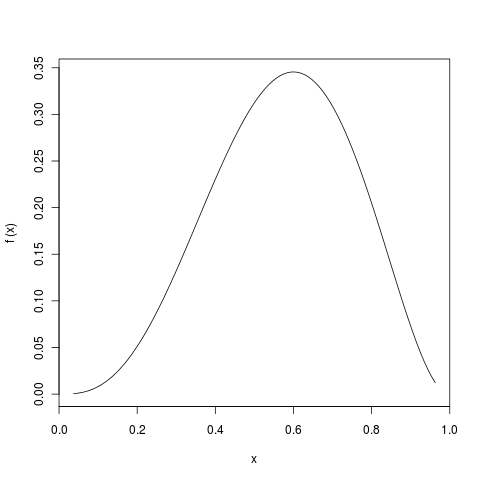
\includegraphics[width=4in, height=4in,]{img/bernlike.pdf}
\caption{Likelihood function for a binomial experiment}
\end{figure}

\end{center}


\item Normal.\\
\label{sec-1_1_1_2}%
Write $X\sim N(\mu,\sigma^2)$. Then 
\[
f(x|\theta) = \frac{1}{\sigma\sqrt{2\pi}}\exp\left[\frac{-(x-\mu)^{2}}{2\sigma^{2}}\right],\quad-\infty<x<\infty.
\]
Here $\theta = (\mu,\sigma^2)$.  The likelihood function is
\begin{eqnarray*}
L(\theta) & = & \prod_{i=1}^{n}\frac{1}{\sigma\sqrt{2\pi}}\exp\left[\frac{-(x_{i}-\mu)^{2}}{2\sigma^{2}}\right]\\
 & = & (2\pi\sigma^{2})^{-n/2}\exp\left[-\frac{1}{2\sigma^{2}}\sum_{i=1}^{n}(x_{i}-\mu)^{2}\right],
\end{eqnarray*}
for $-\infty < \mu < \infty$ and $\sigma > 0$.

\begin{center}

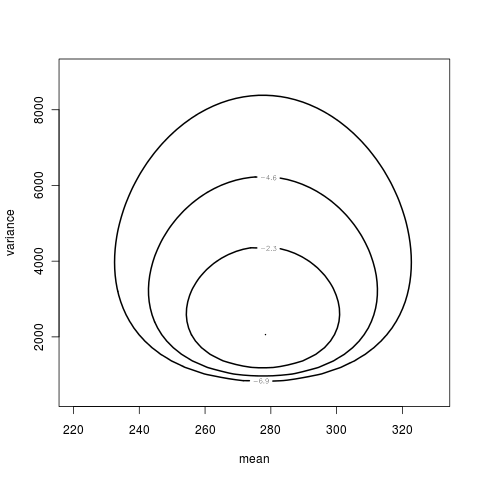
\includegraphics[width=3in, height=3in,]{img/norm2like.pdf}

\end{center}

\end{itemize} % ends low level
\subsection{Statistical Inference}
\label{sec-1_1_2}
\begin{itemize}

\item Point estimation: maximize $L(\theta)$ to get $\hat{\theta}$.\\
\label{sec-1_1_2_1}%
\begin{itemize}
\item \(\hat{\theta}\) is called an ``MLE''.
\end{itemize}

\begin{center}

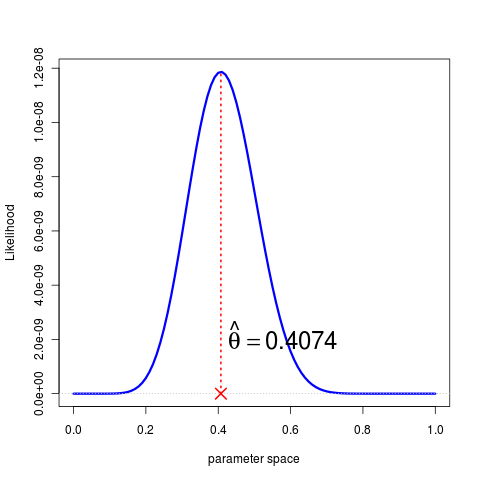
\includegraphics[width=3in, height=3in,]{img/bernMLE.pdf}

\end{center}


\item Interval estimation: use\\
\label{sec-1_1_2_2}%
\[
\hat{\theta} \pm z_{\alpha/2}\cdot \sigma_{\hat{\theta}},
\]
where $\sigma_{\hat{\theta}}$ is the standard error of $\hat{\theta}$ which is $\sqrt{\mathrm{Var}(\hat{\theta})}$.  


\begin{itemize}
\item Usually we don't know $\sigma_{\hat{\theta}}$.  We approximate it.
\item If $l(\theta) = \log L(\theta)$ then when $n$ is large
\end{itemize}
\[
\mathrm{Var}(\hat{\theta}) \approx -\frac{1}{l''(\hat{\theta})}.
\]


\begin{itemize}
\item From a higher class\ldots{} MLEs are aymptotically efficient; use the Delta method.
\end{itemize}

\end{itemize} % ends low level
\subsection{Examples of MLEs}
\label{sec-1_1_3}
\begin{itemize}

\item Bernoulli
\label{sec-1_1_3_1}%
\begin{eqnarray*}
L(\theta) & = & \prod_{i=1}^{n}\theta^{x_{i}}(1-\theta)^{1-x_{i}}\\
 & = & \theta^{\sum x_{i}}(1-\theta)^{n-\sum x_{i}},\quad0<\theta<1.
\end{eqnarray*}

\[
\mathrm{MLE} = \hat{\theta} = \frac{\sum x_{i}}{n} = \xbar. 
\]


\item Bivariate normal
\label{sec-1_1_3_2}%
\begin{eqnarray*}
L(\theta) & = & \prod_{i=1}^{n}\frac{1}{\sigma\sqrt{2\pi}}\exp\left[\frac{-(x_{i}-\mu)^{2}}{2\sigma^{2}}\right]\\
 & = & (2\pi\sigma^{2})^{-n/2}\exp\left[-\frac{1}{2\sigma^{2}}\sum_{i=1}^{n}(x_{i}-\mu)^{2}\right],
\end{eqnarray*}
Can show (see 5844/6944 book)
\[
\frac{\partial}{\partial\mu}l(\theta) = 0 \mbox{ has solution } \hat{\mu}=\xbar,
\]
\[
\frac{\partial}{\partial\sigma^{2}}l(\theta) = 0 \mbox{ has solution } \hat{\sigma^{2}}=\frac{1}{n}\sum_{i=1}^{n}(x_{i} - \xbar)^{2}.
\]

That is, $\hat{\theta} = \left(\xbar,\,n^{-1}\sum_{i=1}^{n}(x_{i} - \xbar)^{2}\right)$.  JOINT MLE.


\item Beta - harder situation, but still possible.\\
\label{sec-1_1_3_3}%
Write $X \sim \mathrm{Beta}(\alpha,\beta)$.
\begin{equation}
f_{X}(x)=\frac{\Gamma(\alpha+\beta)}{\Gamma(\alpha)\Gamma(\beta)}\: x^{\alpha-1}(1-x)^{\beta-1},\quad0 < x <1,
\end{equation}
where $\alpha > 0$ and $\beta > 0$ and
\begin{equation}
\Gamma(\alpha)=\int_{0}^{\infty}x^{\alpha-1}\me^{-x}\:\diff x,\quad\mbox{for }\alpha>0.
\end{equation}



\begin{itemize}
\item Pictures of some Betas.
\end{itemize}

\begin{center}

\begin{figure}[h!]
\centering
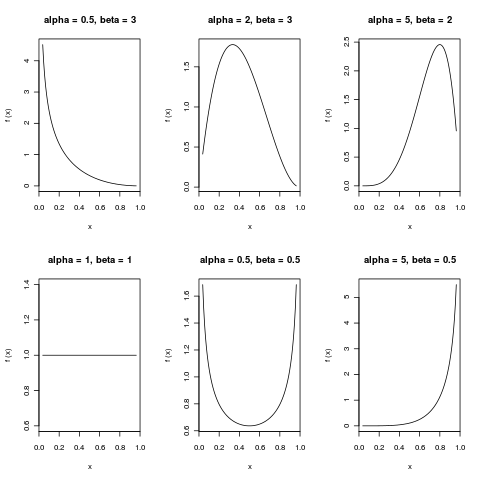
\includegraphics[width=6in, height=6in,]{img/betaexamples.pdf}
\caption{Pictures of some Beta distributions}
\end{figure}

\end{center}

Then 
\[
L(\theta) = \prod_{i=1}^{n}\frac{\Gamma(\alpha+\beta)}{\Gamma(\alpha)\Gamma(\beta)}\: x_{i}^{\alpha-1}(1-x_{i})^{\beta-1}, \quad \alpha > 0,\ \beta > 0.
\]

The likelihood equations simplify to
\[
\begin{cases}
\frac{1}{n}\sum\ln x_{i} & =\Psi(\alpha)-\Psi(\alpha+\beta),\\
\frac{1}{n}\sum\ln(1-x_{i}) & =\Psi(\beta)-\Psi(\alpha+\beta),
\end{cases}
\]
where $\Psi(z)=\Gamma'(z)/\Gamma(z)$ is the \emph{digamma} function.


\begin{itemize}
\item This looks hard!
\begin{itemize}
\item analytically impossible
\item numerically trivial.
\end{itemize}
\end{itemize}

\end{itemize} % ends low level
\section{Why are we in Statistical Computing?}
\label{sec-1_2}


Likelihood functions can be complicated!
\subsection{Censored or missing data}
\label{sec-1_2_1}



\begin{itemize}
\item Data are right censored, say, we are doing a study  about the effectiveness of a drug on a disease.
\item Let \(X_{i} =\) time until onset of disease for \(i^{\mathrm{th}}\) patient, \(i=1,\ldots,n\).
\item Suppose \(X_{1},\ldots X_{n}\) are IID
   \[
   f(x|\theta),\quad \mbox{``survival density''}\quad \mathrm{PDF}
   \]
   \[
   F(x|\theta),\quad \mbox{``survival CDF''},\quad =\int_{-\infty}^{x}f(t|\theta)\diff t
   \]
\item However, the length of the study is LIMITED to $c$ duration (\emph{e.g.} $c=5$ years).
\item The data are  \(X_{1},\ldots X_{n}\), but we actually observe
  \[
  Y_{i}=
  \begin{cases}
  X_{i}, & \mbox{if }X_{i}<c,\\
  c, & \mbox{if }X_{i}\geq c.
  \end{cases}
  \]
\end{itemize}

\begin{center}

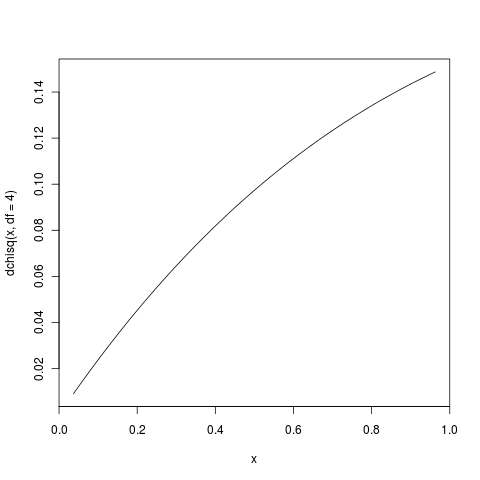
\includegraphics[width=6in, height=3in,]{img/rightcensdata.pdf}

\end{center}


\begin{itemize}
\item Likelihood function
  \[
  L(\theta | y_{1},\ldots,y_{n}) = \prod_{y_{i} < c} f(y_{i}|\theta)\cdot \prod_{y_{i}\geq c}\left[ 1 - F(c|\theta) \right]
  \]
\item This is a typical/common problem.  We will return often.
\end{itemize}
\subsection{Robust modelling/Likelihood can be multimodal}
\label{sec-1_2_2}



\begin{itemize}
\item Typically we assume \(X_{1},\ldots X_{n}\) are IID \(N(\mu,\sigma^{2})\).
\item Then \( L(\mu,\sigma^{2}) = \) EASY.  \(\hat{\mu} = \xbar\).
\item Is this always appropriate?  NO!  Why?
\end{itemize}
\begin{itemize}

\item Alternative (Nonnormal) Models\\
\label{sec-1_2_2_1}%
Often we have heavy-tailed distributions.


\begin{itemize}
\item Student's \emph{t} distribution.  $T(r,\mu,\sigma^2)$
    \begin{equation}
    f(x)=\frac{\Gamma\left[(r+1)/2\right]}{\sigma\sqrt{r\pi}\,\Gamma(r/2)}\left(1+\frac{(x - \mu)^{2}}{\sigma^{2}r}\right)^{-(r+1)/2},\quad-\infty<x<\infty,
    \end{equation}

    where $-\infty < \mu < \infty$, $\sigma > 0$, and $r = 1, 2,\ldots$ are the \emph{degrees of freedom}.
    \begin{center}

    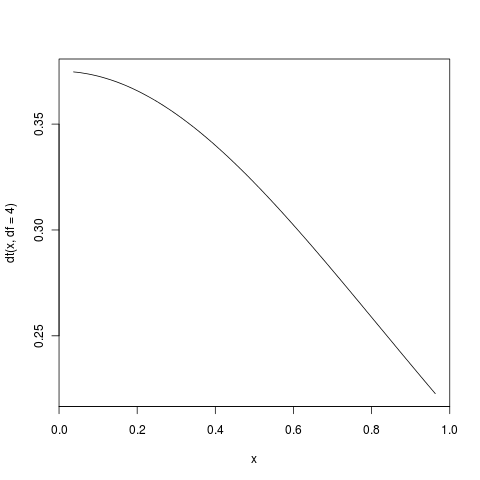
\includegraphics[width=6in, height=3in,]{img/tdistpdf.pdf}

    \end{center}
\begin{itemize}
\item We see that 
    \begin{equation}
    f(x) \propto \sigma^{-1}\left(1+\frac{(x - \mu)^{2}}{\sigma^{2}r}\right)^{-(r+1)/2},
    \end{equation}
\item Usually $r$ is known and $\mu,\sigma^{2}$ are unknown.
\item Given SRS  \(X_{1},\ldots X_{n}\), the likelihood is
    \begin{align*}
    L(\mu,\sigma^{2}) & = \prod \sigma^{-1}\left(1+\frac{(x_{i} - \mu)^{2}}{\sigma^{2}r}\right)^{-(r+1)/2}\\
    & =  \sigma^{-n} \left[\prod \left(1+\frac{(x_{i} - \mu)^{2}}{\sigma^{2}r}\right) \right]^{-(r+1)/2}
    \end{align*}
\item For fixed $\sigma$, by playing with the data one can choose the number of modes of the likelihood.  Notice the inside is a polynomial in $\mu$ of degree $2n$.  It may have many (up to $n$) minima.  Then the likelihood has $n$ maxima, each of which has to be checked.  As $n \to \infty$, this is very difficult.
\end{itemize}
\end{itemize}

\begin{itemize}
\item Cauchy distribution (take $r = 1$ in Student's \emph{t}).
\begin{itemize}
\item Write \(X_{1},\ldots X_{n} \sim \mathrm{Cauchy}(m,\sigma)\), where $m$ is the median and $\sigma$ is a scale parameter.
\item The PDF is 
    \begin{equation}
    f(x|m,\sigma)=\frac{1}{\sigma\pi}\left[1+\left(\frac{x-m}{\sigma}\right)^{2}\right]^{-1},\quad -\infty < x <\infty,
    \end{equation}
    where $-\infty < m < \infty$ and $\sigma > 0$.
\item We use the median and scale parameter because the mean and variance DNE! (it's \emph{very} heavy-tailed.)
    \begin{center}

    \includegraphics[width=4in, height=4in,]{img/cauchydistpdf.pdf}

    \end{center}
\end{itemize}
\end{itemize}


\begin{itemize}
\item Double Exponential (AKA Laplace).
    \begin{equation}
    f(x|\mu,\sigma)=\frac{1}{2\sigma}\exp\left(-\frac{|x - \mu|}{\sigma}\right),\quad -\infty < x <\infty,
    \end{equation}
    where $-\infty < \mu < \infty$ and $\sigma > 0$.
\begin{itemize}
\item the MLE is \(\hat{\mu} = \mathrm{sample median}\)
    \begin{center}

    \includegraphics[width=6in, height=3in,]{img/laplacedistpdf.pdf}

    \end{center}
\end{itemize}
\end{itemize}

\end{itemize} % ends low level
\subsection{Mixture distributions}
\label{sec-1_2_3}

Here we have \(X_{1},\ldots, X_{n} \sim f(x|\theta)\), but $f$ takes the form
\[
f(x|\theta) = \sum_{j=1}^{k}p_{j}f_{j}(x|\theta_{j}),
\]
where $p_{j}\geq 0$ and \(\sum_{j}p_{j}=1\).


\begin{itemize}
\item Have $k$ different groups/subpopulations
\begin{itemize}
\item the proportion of people in group $j$ is $p_{j}$
\item the $j^{\mathrm{th}}$ subpop. has distribution $f_{j}(\cdot |\theta_{j})$
\end{itemize}
\end{itemize}
\begin{itemize}

\item Example: Studying heights of students\\
\label{sec-1_2_3_1}%
\begin{itemize}
\item Let \(X = \mbox{height in inches}  \).
\item Male heights $\approx N(71, 3^2)$
\item Female heights $\approx N(63, 2^2)$
\item Suppose there are 66\% males, 34\% females
\end{itemize}

\begin{center}

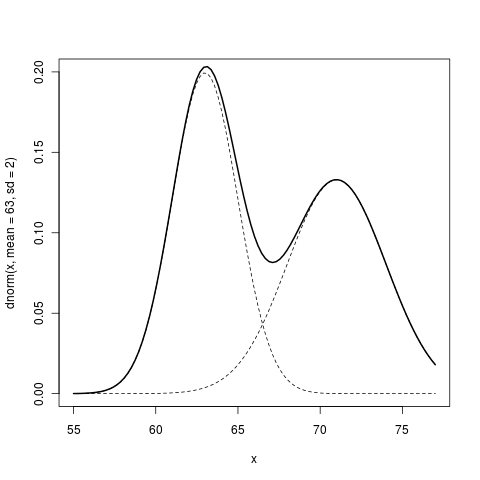
\includegraphics[width=6in, height=3in,]{img/normalmix.pdf}

\end{center}

Then the population density is 

\begin{eqnarray*}
f(x) & = & p\,N(\mu_{1},\sigma_{1}^{2}) + (1 - p)\,N(\mu_{2},\sigma_{2}^{2})\\
     & \approx & 0.66\,f(x|71, 3^{2}) + 0.34\,f(x|63,2^{2})
\end{eqnarray*}

In general, the likelihood is 

\begin{eqnarray*}
L(\theta) & = & \prod_{i=1}^{n} \left( \sum_{j=1}^{k}p_{j}f_{j}(x_{i}|\theta_{j}) \right) \\
     & = & \prod_{i=1}^{n} \left( p_{1}f_{1}(x_{i}|\theta_{1}) + \cdots + p_{1}f_{k}(x_{i}|\theta_{k}) \right)
\end{eqnarray*}
The product, when expanded, will have $k^{n}$ terms.  This explodes as $n \to \infty$, so not only do we have multimodality, we have SMALL RESOURCES, too.

\end{itemize} % ends low level
\subsection{Dependent Bernoulli trials}
\label{sec-1_2_4}

YET ANOTHER MODEL!


\begin{itemize}
\item Coin tossing model: \(X_{1},\ldots, X_{n}\) IID Bern($p$), where
\begin{itemize}
\item $\P(\mbox{success}) = p$, constant, and
\item the trials are independent.
\end{itemize}
\end{itemize}
\begin{itemize}

\item BUT -\\
\label{sec-1_2_4_1}%
\begin{itemize}
\item Maybe the $p$'s change across trials
\item Maybe there is dependence in the sequence
\end{itemize}

Suppose we have belief in STREAKY behavior

\begin{itemize}
\item Two (2) states:
\begin{itemize}
\item $p_{H} \to \mbox{hot state}$
\item $p_{C} \to \mbox{cold state}$
\end{itemize}
\end{itemize}

If you are hot, you are more likely to stay hot in the next trial\ldots{}


\begin{center}
\begin{tabular}{llll}
 Trial  &  $i + 1$  &  hot     &  cold          \\
\hline
 $i$    &           &          &                \\
 hot    &           &  $0.9a$  &  $0.1(1 - a)$  \\
 cold   &           &  0.1     &  0.9           \\
\end{tabular}
\end{center}




\begin{itemize}
\item We don't know: $p_{H}$, $p_{C}$, $a$.
\item Observe a vector of $X$'s, for example,
  \[
  x = (1,1,1,0,0,1,0,0,0,1,0,0,1,1,1)
  \]
\item One possible configuration of states
  \[
  s = (H,H,H,C,C,H,C,C,C,H,C,C,H,H,H)
  \]
\item Probability in this configuration would be
  \[
  \frac{1}{2}p_{H}ap_{H}ap_{H}a(1-a)p_{C}(1-a)p_{C}\cdots
  \]
\end{itemize}

The Likelihood is
\[
L(p_{H},p_{C},a) = \sum_{\mbox{all possible configurations}}\P(\mbox{observe $x$}|\mbox{state is $s$})
\]

\begin{itemize}
\item AKA ``Markov Switching Model''
\item Number of terms in above sum: $2^{n}$ - very complicated.
\end{itemize}

\end{itemize} % ends low level
\section{Introduction to Bayesian Statistics}
\label{sec-1_3}


\begin{itemize}
\item Named for Reverend Thomas Bayes (1702-1761)
\item Based on the theory of subjective probability
\end{itemize}
\subsection{Central Theme}
\label{sec-1_3_1}


\begin{itemize}
\item the quantity of interest, $\theta$, is unknown and considered to be a \emph{random variable}.
\item we have beliefs / existing knowledge about $\theta$, represented by
  \[
  \pi(\theta) \leadsto \mbox{the \textbf{PRIOR distribution} of $\theta$.}
  \]
\item $\pi$ is a PDF, nonnegative, integral one.
\end{itemize}
We wish to learn about \(\theta\)! To this end we conduct an experiment, and consequently we observe a random variable $X$ which depends (in some way) on $\theta$. The conditional distribution of $X$ given $\theta$ is represented by
\[
f(x|\theta) \leadsto \mbox{ the \textbf{LIKELIHOOD function}}.
\]
We wish to UPDATE our beliefs about $\theta$, using the information contained in the observation $X=x$ combined with our prior beliefs. Our new beliefs will be represented by
\[
\pi(\theta|x) \leadsto \mbox{the \textbf{POSTERIOR distribution} of $\theta$.}
\]


\begin{description}
\item[Method:] BAYES' RULE
\end{description}

\[
\pi(\theta|x)=\frac{f(x|\theta)\, \pi(\theta)}{\int f(x|\theta)\, \pi(\theta)
\diff\theta}, \quad \mbox{for $\theta \in \Theta$.}
\]
\begin{itemize}

\item Remarks:\\
\label{sec-1_3_1_1}%
\begin{itemize}
\item Once beliefs are updated, we then go out and do another experiment to learn even more!  Update again.  Schematic Diagram.
\item From Bayes' Rule
   \begin{align*}
   \pi(\theta|x)&=\frac{f(x|\theta)\, \pi(\theta)}
   {\int f(x|\theta)\, \pi(\theta)d\theta}\\
   &= M \, f(x|\theta)\, \pi(\theta)\\
   &\propto f(x|\theta)\, \pi(\theta).
   \end{align*}
   Hence, Bayes' Rule is often written in the form POSTERIOR $\propto$ LIKELIHOOD $\times$ PRIOR
\item Notice the difference in interpretations:
   For a Frequentist:
   \[
   \mbox{LIKELIHOOD}=L(\theta)=f(\mathbf{x}|\,\theta)= \mbox{a function of $\theta$}.
   \]
   While for a Bayesian:
   \[
   \mbox{LIKELIHOOD}=f(\mathbf{x}|\,\theta)= \mbox{a function of $\mathbf{x}$}.
   \]
\end{itemize}


\item Examples.\\
\label{sec-1_3_1_2}%
Want to learn about
\[
p = \mbox{proportion of goldfish in lake}
\]


\begin{enumerate}
\item Construct a continuous prior for $p$.

   \begin{center}

   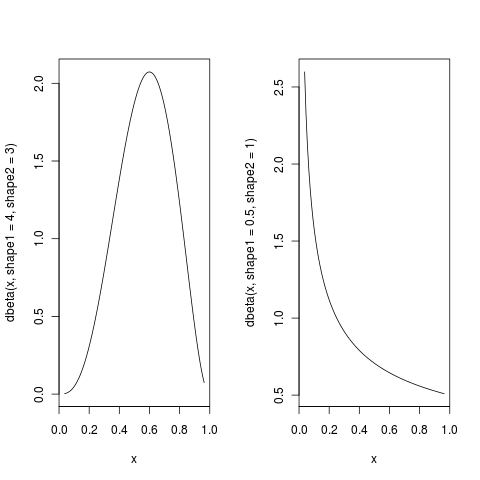
\includegraphics[width=6in, height=3in,]{img/fishprior.pdf}

   \end{center}
   Let $p$ have a Beta density,
   \begin{equation}
   p \sim \pi(p)=\frac{\Gamma(\alpha+\beta)}{\Gamma(\alpha)\Gamma(\beta)}\: p^{\alpha-1}(1-p)^{\beta-1},\quad 0 < p < 1. \quad \mbox {This is the prior.}
   \end{equation}
\begin{itemize}
\item Some properties
\begin{enumerate}
\item \(\E[p] = \frac{\alpha}{\alpha+\beta}=\eta  \)
\item \(\mbox{Var}(p) = \frac{\eta(1 - \eta)}{\alpha + \beta + 1} = \frac{\alpha\beta}{(\alpha + \beta)^{2}(\alpha + \beta + 1)}   \)
\item Think of $\eta$ as a \emph{prior guess} at $p$
\item Think of \(\kappa = \alpha + \beta\) as \emph{precision} of belief
\item The CDF is
\end{enumerate}
\[
      \P(p \leq x) = \int_{0}^{x}\frac{\Gamma(\alpha+\beta)}{\Gamma(\alpha)\Gamma(\beta)}\: p^{\alpha-1}(1-p)^{\beta-1}\,\diff p.
      \]
      The above is the \emph{incomplete beta function}.
\end{itemize}
\item Want to learn about $p$:  Go fishing! We catch $n$ fish, and let
   \[
   Y = \mbox{number of goldfish caught.} 
   \]
   Then \( Y = X_{1}+\cdots+X_{n} \), where 
   \[
   X_{i}=
   \begin{cases}
   1, & \mbox{if $i^{\mathrm{th}}$ fish is a goldfish},\\
   0, & \mbox{otherwise}.
   \end{cases}
   \]
   So \(X_{i} \sim \mathrm{Bern}(p)\).  Then \(Y \sim \mathrm{Binom}(p)\) with
   \[
   f(y|p) = {n \choose y}\,p^{y}(1-p)^{n - y},\quad y = 1,2,\ldots,n. \quad \mbox{(this is the Likelihood)}
   \]
\item Update beliefs with Bayes' Rule.
   \[
   \mbox{POSTERIOR \(\propto\) LIKELIHOOD $\times$ PRIOR}
   \]
   This means
   \begin{align*}
   \pi(\theta|y)& \propto f(y|p) \times \pi(p)\\
   &= {n \choose y}\,p^{y}(1 - p)^{n - y}\frac{\Gamma(\alpha+\beta)}{\Gamma(\alpha)\Gamma(\beta)}\: p^{\alpha-1}(1-p)^{\beta-1}\\
   &= M \cdot p^{\alpha + y - 1}\cdot (1 - p)^{\beta + n - y - 1}.
   \end{align*}
   where $M$ is such that
   \[
   \int_{0}^{1}\pi(p|y)\,\diff p = 1.
   \]
   By inspection, we see that
   \[
   p|y \sim \mathrm{Beta}(\alpha + y,\beta + n- y),
   \]
   and so we conclude
   \begin{align*}
   M &= \frac{\Gamma((\alpha + y)+(\beta+n-y))}{\Gamma(\alpha+y)\Gamma(\beta+n-y)},\\
   &= \frac{\Gamma(\alpha+\beta+n)}{\Gamma(\alpha+y)\Gamma(\beta+n-y)}.
   \end{align*}

   \textbf{Summary:}
\begin{itemize}
\item Started with prior, \(p \sim \mathrm{Beta}(\alpha,\beta).  \)
\item Did experiment, observed $Y = y$.
\item Get posterior, \(p|y \sim \mathrm{Beta}(\alpha + y,\ \beta + n - y).  \)
\end{itemize}
\end{enumerate}

\end{itemize} % ends low level
\subsection{Bayesian Statistics}
\label{sec-1_3_2}

Draw all inference from the posterior distribution $\mathrm{Beta}(\alpha + y,\ \beta + n - y)$.

Our new guess at $p$:
\begin{align*}
\eta^{\ast} &= \frac{\alpha^{\ast}}{\alpha^{\ast}+\beta^{\ast}} \\
&= \frac{\alpha + y}{(\alpha + y) + (\beta + n - y)} \\
&= \frac{\alpha + y}{\alpha + \beta + n} \\
&= \frac{\alpha}{\alpha + \beta + n}\cdot\frac{\alpha + \beta}{\alpha + \beta} + \frac{y}{\alpha + \beta + n}\cdot\frac{n}{n} \\
&= \frac{\alpha}{\alpha + \beta}\cdot\frac{\alpha + \beta}{\alpha + \beta + n} + \frac{y}{n}\cdot\frac{n}{\alpha + \beta + n} \\
&= \eta\cdot\frac{\kappa}{\kappa + n} + \frac{y}{n}\cdot\frac{n}{\kappa + n}
\end{align*}

That is, the POSTERIOR MEAN is a \emph{weighted average} or the MLE and the PRIOR MEAN.  It's called a \emph{shrinkage estimator}.


\begin{itemize}
\item As $\kappa \to \infty$, we have $\eta^{\ast} \to \eta$.
\item As $n \to \infty$, we have $\eta^{\ast} \to \mathrm{MLE}$.
\end{itemize}

\textbf{Remarks:}
\begin{itemize}

\item How do we choose a prior?\\
\label{sec-1_3_2_1}%
Notice:

\begin{itemize}
\item Prior $\to$ Beta
\item Posterior $\to$ Beta, too.
\end{itemize}

\(\mathrm{Beta}(\alpha,\beta)\) is called a CONJUGATE FAMILY.

Beta/Binomial is called a CONJUGATE PAIR.

Another conjugate pair: if \(\pi(\theta) = N(\mu,\,\tau^{2})\) and  \(f(x|\theta) = N(\theta,\,\sigma^{2})\), then
\[
\pi(\theta|x) = N\left(\frac{\xbar\tau^{2}+\mu\sigma^{2}/n}{\tau^{2}+\sigma^{2}/n},\,\frac{\tau^{2}\cdot\sigma^{2}/n}{\tau^{2}+\sigma^{2}/n}  \right).
\]


\begin{itemize}
\item Other pairs:
\begin{itemize}
\item Gamma/Normal
\item Gamma/Poisson
\item Gamma/Gamma
\end{itemize}
\end{itemize}

Here, \(\mathrm{Gamma}(\alpha,\beta)\) has PDF
\[
f(x|\alpha,\beta) = \frac{1}{\Gamma(\alpha)\beta^{\alpha}}\,x^{\alpha - 1} \me^{-x/\beta},\ x > 0,
\]
where $\alpha > 0$ and $\beta > 0$.

Special cases:

\begin{itemize}
\item \(\mathrm{Exp}(\beta) = \mathrm{Gamma}(1,\beta)\)
\item Chi-square \(\chi^{2}(\nu) = \mathrm{Gamma}(\nu/2,\,2),\ \nu =1,2,\ldots\)
\end{itemize}

Conjugate families were chosen for priors historically because they are traqctable, convenient, easy.  Turns out, conjugate families are \emph{very} restricted (that is, most families of priors are not conjugate).  This used to be a problem, but computing advances have made this last difficulty negligible.


\item Bayesian Point Estimation\\
\label{sec-1_3_2_2}%
Our new guess at $\theta$:  the POSTERIOR MEAN $\E [\theta|x]$.

Fact: the posterior mean is optimal in almost every sense, under the assumption of \emph{squared error loss}.

The squared error loss of an estimator $\delta$ which estimates $\theta$ is 
\[
L(\delta,\theta) = (\delta - \theta)^{2}.
\]

We will often need to compute the posterior mean.  Therefore we will need to compute things like
\begin{align*}
\E [\theta|x] &= \int \, \theta\, \pi(\theta|x)\,\diff \theta,  \\
&= \int \frac{\theta\, f(x|\theta)\,\pi(\theta)}{\int f(x|u)\pi(u)\diff u} \,\diff \theta, \\
&= M \cdot \int \theta f(x|\theta)\pi(\theta)\,\diff \theta.
\end{align*}

This will often be complicated, with no closed form solution.  Therefore we will need to resort to computing techniques.


\item Bayesian Interval Estimation\\
\label{sec-1_3_2_3}%
Here we have a probability interval of probability content $\gamma$, AKA ``credible regions''.

The Bayesian has many options:


\begin{itemize}
\item Equal-Tails interval
\item Shortest interval of content $\gamma$, or ``HDR (highest density region)'' interval
\end{itemize}

Since posteriors are often complicated, calculation of credible regions is difficult and we need Monte Carlo techniques.


\end{itemize} % ends low level
\chapter{Random Variable Generation}
\label{sec-2}

We will talk about the following:


\begin{itemize}
\item Basic Methods: generating pseudo-random uniform numbers
\item Linear Congruential and Shift Register generators
\item Generating non-uniforms
\item Accept – Reject Methods
\end{itemize}
\section{Basic Methods: generating pseudo-random uniform numbers}
\label{sec-2_1}
\subsection{Desires for a Uniform Pseudo-Random Generator}
\label{sec-2_1_1}


\begin{enumerate}
\item Want the distribution of the numbers to be uniform
\item Want independence of variates
\item Should be repeatable, portable
\item High computational speed
\end{enumerate}

\textbf{Repeatability:} the ability to repeat the same stream of numbers at any time during the simulation. Useful for comparing simulations using different methods.
\subsection{History}
\label{sec-2_1_2}

Guiding principle is that the validity of any simulation rests on the validity of the uniform generator.

People first used ``random sources'' to supply random numbers.

\begin{itemize}
\item census reports
\item mechanical devices
\item drums, ping-pong balls in state lotteries
\item Famous random number tables (tables with over a million numbers)
\end{itemize}

We use an algorithm to generate pseudo-random numbers. We call it random since the output resembles a random sequence, at least in the sense that it passes standard statistical tests of randomness. But we will be using a deterministic sequence to generate/simulate a ``random'' sequence.
\subsection{Early Method: von Neumann's Midsquare Method}
\label{sec-2_1_3}


Generates a random integer between 0 and 99,999.


\begin{enumerate}
\item Choose any 5-digit number as the seed (12345)
\item Square seed and add leading zeros, to make it 10 digits (0152399025)
\item Take 3-7 digits as your random number (52399)
\end{enumerate}

We want values uniformly distributed. Since the method is iterative, the sequence will eventually repeat in cycles. For poor choices of the seed, unfortunately, the cycle length can be very short.

The output CAN behave ``randomly'', but how do we know? To statistically check apparent randomness we could use a Chi-Square Goodness of Fit test:

\begin{itemize}
\item Generate 5000 values, normalize by dividing by 100,000
\item Hypothesis: $X_{1},X_{2},\ldots,X_{5000}\sim\mathrm{Unif}(0,1)$
\item Partition \( [0,1] \) into, say, 10 intervals and calculate frequencies $f_{1},f_{2},\ldots,f_{10}$
\item Compute the statistic: $\chi^{2}=\sum(O_{i}-E_{i})^{2}/E_{i}$
\end{itemize}
\section{Linear Congruential and Shift Register Generators}
\label{sec-2_2}


In current algorithms, most generators generate pseudo-random 32-bit integers.  
\subsection{Congruential algorithm:}
\label{sec-2_2_1}

Based on the formula 
\[
U_{i}=(aU_{i-1}+c)\mod m,
\]
where $U_{i}$ is the random integer, $U_{0}$ is the seed, and $a,c,m$ are selected constants.


\begin{description}
\item[Properties:] of the congruential algorithm
\begin{enumerate}
\item Generates values $0,1,\ldots,m-1$.
\item After some iterations the sequence will repeat, and the length of the sequence is the \emph{period}.
\item The maximum period is $m$.
\item If we want Unif(0,1) numbers, we will get values $0/m,1/m,\ldots,(m-1)/m$.
\item Problem is how to choose $a,c,m$. This determines the number of possible uniforms and period.
\end{enumerate}
\item[NUMBER THEORY RESULTS:] Choosing $a,c,m$.
\begin{itemize}
\item Choose $m$ as large as possible.
\item Given $m$, the constants $a$ and $c$ can be chosen such that the period is $m$.
\end{itemize}
\item\textbf{Result:} A linear congruential generator has maximal cycle length $m$ if and only if:
\begin{itemize}
\item $c$ is nonzero and relatively prime to $m$.
\item \( (a\mod q) = 1 \) for each prime factor $q$ of $m$.
\item \( (a\mod 4) = 1 \) if 4 is a factor of $m$.
\end{itemize}
\end{description}

Researchers have found values of $a,c,m$ which give a long period and appear to be uniformly distributed.


\begin{description}
\item[Bad Generator:] RANDU.  
  \[
  c = 0,\quad a=2^{16}+3,\quad m=2^{31}
  \]
  This generator is very fast, but has poor statistical properties. In particular, $U_{i}$ and $U_{i+2}$ are highly positively correlated.

   \begin{center}

   \includegraphics[width=6in, height=6in,]{img/randu.pdf}

   \end{center}
\end{description}

\vspace{1in}


\begin{description}
\item[Good Generator:] here's one: 
  \[
  U_{i}=(16,807U_{i-1})\mod(2^{31}-1),
  \]
  It's good because:
\begin{itemize}
\item simple
\item widespread use
\item long cycle length $2^{31}-2$ (all numbers besides 0 and $2^{31}-1$ can be generated).
\end{itemize}
\end{description}
\subsection{Shift Register generators}
\label{sec-2_2_2}

These operate on \emph{n}-bit pseudo-random binary vectors.

\begin{itemize}
\item \textbf{Example:} Generate a random 7 bit vector.
\begin{enumerate}
\item Choose a seed. (1001101)
\item Shift it to the right by 2 units. (0010011)
\item Add lines 1) and 2). (1011110)
\item Shift sum to the left by three bits. (1110000)
\item Add lines 3) and 4). \textbf{Result} (0101110)
\end{enumerate}
\end{itemize}

Parameters of the algorithm: 

\begin{itemize}
\item the length of the binary vector,
\item the shift right length, and
\item the shift left length.
\end{itemize}

This is a popular algorithm\ldots{} why? Because it is easy to implement on a computer! One can have hybrid methods, or those that combine several methods. A popular one is the KISS algorithm (Keep it simple, stupid!)
\section{Generating Non-Uniform Random Numbers}
\label{sec-2_3}


There are three general methods: 

\begin{enumerate}
\item CDF Inversion,
\item Transformations, and
\item Accept/Reject methods.
\end{enumerate}
\subsection{CDF Inversion}
\label{sec-2_3_1}


The inversion method is based on the following.


\begin{description}
\item[Probability Integral Transformation:] Suppose \(X\) has a continuous strictly increasing CDF $F_{X}(x)=\P(X \leq x)$. Denote the inverse CDF $F_{X}^{-1}(y)$.  If $U\sim\mathrm{Unif}(0,1)$, then $F_{X}^{-1}(U)$ is distributed according to $F_{X}$.
\item[Proof:] Let \(Y = F_{X}^{-1}(U)\). Then 
  \[
  \P(Y \leq y)=\P(F_{X}^{-1}(U)\leq y)=\P(U\leq F_{X}(y)).
  \]
  But a Unif(0,1) random variable satisfies $\P(\mbox{uniform}\leq x) = x$, and we are done.
\end{description}

Thus, if we can find $F_{X}^{-1}$, the inverse CDF, all we have to do is apply $F_{X}^{-1}(U)$ to a uniform $U$ to get random numbers from $F_{X}$.


\begin{description}
\item[Note:] We assumed above that the CDF was strictly increasing, but we didn't need to\ldots{} the statement is true for any continuous CDF. In the general case we must define 
  \[
  F_{X}^{-1}(t)=\inf\{x:\ F_{X}(x)\geq t\}.
  \]
\end{description}
\begin{itemize}

\item Example. Exponential. \(\mathrm{Exp}(\theta)\).\\
\label{sec-2_3_1_1}%
$X$ has $f(x)=\frac{1}{\theta}\, \me^{-x/\theta}$, $x > 0$.  The CDF is $\P(X\leq x)=1 - \me^{-x/\theta}$, $x > 0$. Now set $F_{X}(x) = y$, and solve for $x$. 
\begin{align*}
1 - \me^{-x/\theta} & = y\\
\me^{-x/\theta} & = 1 - y\\
-x/\theta & = \ln(1-y)\\
x & = -\theta\ln(1-y) = F_{X}^{-1}(y).
\end{align*}

\textbf{R code:} To generate 100 Exp(1)'s: write
\begin{verbatim}
u <- runif(100)
x <- -log(1 - u)
\end{verbatim}

Or we could do it more directly with
\begin{verbatim}
x <- rexp(100)
x <- rexp(100, scale = theta)
\end{verbatim}


\textbf{Note:} If \(U\sim \mathrm{Unif}(0,1)\), then \( (1-U)\sim \mathrm{Unif}(0,1) \). Therefore, \(-\log(1-(1-U))\sim \mathrm{Exp}(1)\), that is, \(-\log(U)\sim \mathrm{Exp}(1)\).

\textbf{Example.} Logistic (standard). \( \mathrm{Logis}(0,1) \)
\[
f(x)=\frac{\me^{-x}}{(1 + \me^{-x})^{2}},\quad -\infty < x <\infty.
\]
and 
\[
F(x)=\frac{\me^{x}}{1 + \me^{x}} = y
\]
\begin{center}

\includegraphics[width=4in, height=4in,]{img/logisdistpdf.pdf}

\end{center}
Solving for $x$, 
\begin{align*}
\me^{x} & = y(1 + \me^{x})\\
\me^{x}(1-y) & = y\\
\me^{x} & = \frac{y}{1 - y} \\
x & = \ln \frac{y}{1 - y} = F_{X}^{-1}(y) = \mbox{logit}\ y.
\end{align*}

Therefore, to generate standard Logistic, we could do
\begin{verbatim}
u <- runif(100)
x <- log(u/(1 - u))
\end{verbatim}

Or we could do it more directly in \texttt{R} with
\begin{verbatim}
x <- rlogis(100)
\end{verbatim}


\textbf{Example.} Normal, \( N(\mu,\sigma^{2}) \). 
\[
F(x)=\int_{-\infty}^{x}\frac{1}{\sigma\sqrt{2\pi}}\exp\{\frac{-1}{2\sigma^{2}}(t-\mu)^{2}\}\:\diff t
\]

This function doesn't have a closed form representation, yet we can approximate $F$ and $F^{-1}$ arbitrarily closely with numerical methods. For example, for $N(0,1)$ we have 
\[
\Phi^{-1}(\alpha)\approx t-\frac{a_{0}+a_{1}t}{1+b_{1}t+b_{2}t^{2}},
\]
where $t^{2}=\log(\alpha^{-2})$ and 
\[
\begin{array}{cccc}
a_{0}=2.30753, & a_{1}=0.27061, & b_{1}=0.99229, & b_{2}=0.04481.
\end{array}
\]
 These are accurate up to order \(10^{-8}\). This sounds good, but we can do BETTER!

\end{itemize} % ends low level
\subsection{Transformation Methods}
\label{sec-2_3_2}



\begin{description}
\item[Location-Scale families:] here the family of PDFs $f(x|\theta),\ \theta\in\Theta$ are of the form 
  \[
  f(x|\mu,\sigma)=\frac{1}{\sigma}h\left(\frac{x-\mu}{\sigma}\right),
  \]
  for some PDF $h$. If it is desired to generate an RV $X\sim f(\cdot|\mu,\sigma)$, then it is only necessary to generate $V\sim f(\cdot|0,1)$, for then we make the transformation 
  \[
  X = \mu + \sigma V.
  \]
  By a change of variables, \( X \sim f(\cdot|\mu,\sigma) \).
\end{description}
\begin{itemize}

\item Example. Logistic. \( \mathrm{Logis}(\mu,\beta) \).\\
\label{sec-2_3_2_1}%
If \( Y \sim \mathrm{Logis}(\mu,\beta) \) then $Y$ has PDF
\[
f_{Y}(y)=\frac{1}{\beta}\frac{\me^{-\frac{y-\mu}{\beta}}}{(1 + \me^{-\frac{y-\mu}{\beta}})^{2}},\quad -\infty< y <\infty.
\]
To generate 100 IID $Y$'s distributed Logis(3,7) we may use the \texttt{R} code:

\begin{verbatim}
u <- runif(100)   # 100 uniforms
x <- log(u(1-u))  # 100 std logistics
y <- 3 + 0.7*x    # 100 Log(3,7)'s
\end{verbatim}

or more directly with \texttt{R} we could do
\begin{verbatim}
rlogis(100, location = 3, scale = 7)  # location/scale logistics
\end{verbatim}


\begin{description}
\item[Using Exponentials to build other distributions] Example: Generating Gammas.
\item[Know:] If \(U \sim\mathrm{Unif}(0,1)\), then \( -\theta\log(U)\sim\mathrm{Exp}(\theta) \).
\item[Know:] Let $X_{1},X_{2},\ldots,X_{n}\sim\mathrm{Exp}(\theta)$ be IID.  Let $Y=\sum_{i}X_{i}$. Then $Y\sim\mathrm{Gamma}(n,\theta)$.
\end{description}

\textbf{R:} To simulate \( \mathrm{Gamma}(n,\theta) \):
\begin{verbatim}
u <- runif(n)             # n uniforms
x <- -theta * log(u)      # n Exp(theta)s
y <- sum(x)               # a gamma(n, theta)
\end{verbatim}

A shorter way would be:
\begin{verbatim}
u <- sum(-theta * log(runif(n)))
\end{verbatim}

This only works for $n$ = a positive integer. We would need another algorithm for non-integral $n$, but with \texttt{R} we can do whatever we want.
\begin{verbatim}
u <- rgamma(1, shape = n, scale = theta)
\end{verbatim}

Note that above we would change the first argument, \texttt{1}, to however many gammas we like.


\textbf{Example.} Generating Betas.


\begin{description}
\item[Know:] If \( U\sim\mathrm{Gamma}(\alpha,1)\) and \(V\sim\mathrm{Gamma}(\beta,1)\), then \(\frac{U}{U+V}\sim\mathrm{Beta}(\alpha,\beta)\).
\end{description}

\textbf{R:} To simulate $\mathrm{Beta}(m,n)$:
\begin{verbatim}
u <- sum(-log(runif(m)))     # a Gamma(a,1)
v <- sum(-log(runif(n)))     # a Gamma(b,1)
y <- u/(u+v)                 # a Beta(a,b)
\end{verbatim}

Unfortunately, this method only works for integral $\alpha$ and $\beta$.  When we do it with \texttt{R} directly we can use whatever we like:
\begin{verbatim}
u <- rbeta(1, shape1 = a, shape2 = b)
\end{verbatim}


\textbf{Example.} Generating Chi-Squares.


\begin{description}
\item[Know:] $\chi^{2}(\nu)=\mathrm{Gamma}(\nu/2,2)$.
\end{description}

\textbf{R:} To simulate $\chi^{2}(2k)$:
\begin{verbatim}
y <- sum(-2*log(runif(k)))   # a Gamma(k,2)
y <- rchisq(1, df = k)       # same thing
\end{verbatim}

This only works for even degrees of freedom, unfortunately. When we do it with \texttt{R} directly we can use whatever we like:
\begin{verbatim}
u <- rchisq(500, df = m)
\end{verbatim}


\textbf{Example.} Generating Fs.


\begin{description}
\item[Know:] Snedecor's $F$ distribution $F(\alpha,\beta)$.
  \[
  f(x|\alpha,\beta)=\frac{\Gamma((\alpha+\beta)/2)\alpha^{\beta/2}\beta^{\alpha/2}}{\Gamma(\alpha/2)\Gamma(\beta/2)}\frac{x^{(\alpha-2)/2}}{(\alpha+\beta x)^{(\alpha+\beta)/2}},\quad x>0,\quad\alpha,\beta>0.
  \]
\item[Know:] If $U\sim\chi^{2}(m)$ and $V\sim\chi^{2}(n)$ are independent, then $\frac{U/m}{V/n}\sim F(m,n)$.
\end{description}

\textbf{R:} To simulate $F(2k,2l)$:
\begin{verbatim}
u <- sum(-2*log(runif(k)))        # a Chi-square(2k)
v <- sum(-log(runif(a)))          # a Chi-square(2l)
y <- (u/k)/(v/l)                  # an F(2k,2l)
\end{verbatim}

Again, the above method will only work for even degrees of freedom but the direct method can do anything.
\begin{verbatim}
y <- rf(500, df1 = m, df2 = n)    # 500 F(m,n)'s
\end{verbatim}
 


\textbf{Using the Order statistics.}


\begin{description}
\item[Know:] Let $X_{1},X_{2},\ldots,X_{n}$ be IID from a continuous population with PDF $f(x)$ and CDF $F(x)$. Denote the order statistics by $X_{(1)}\leq X_{(2)}\leq\cdots\leq X_{(n)}$. Then the p.d.f.\textbackslash{} of $X_{(k)}$ is 
  \[
  f_{X_{(k)}}(x)=\frac{n!}{(k-1)!(n-k)!}[F(x)]^{k-1}f(x)[1-F(x)]^{n-k}.
  \]
\end{description}
\textbf{Special Case:} $f(x)=1$, $0 < x < 1$.   Then $F(x)=x$ and the above simplifies to 
\[
X_{(k)}\sim f_{X_{(k)}}(x)=\frac{n!}{(k-1)!(n-k)!}\, x^{k-1}\,(1-x)^{n-k},
\]
which is a $\mathrm{Beta(k,\,n-k+1)}$ distribution.

\textbf{R:} An alternative to simulate $\mathrm{Beta}(k,\,n-k+1)$:

\begin{verbatim}
u <- runif(n)  # n uniforms
v <- sort(u)   # order the uniforms
y <- v[k]      # the kth order statistic
\end{verbatim}

This algorithm is costly for large $k$ and $n$, since sorting a vector is often difficult for computers.


\textbf{Example.} Generating \(N(0,1)\) \emph{exactly}.


\begin{description}
\item[Know:] If $X_{1}$ and $X_{2}$ are i.i.d. $N(0,1)$, then the point $(X_{1},X_{2})$ in the Cartesian plane satisfies
\begin{itemize}
\item $r^{2}=X_{1}+X_{2}\sim\chi^{2}(2)$.
\item $\theta \sim \mathrm{Unif}(0,2\pi)$.
\item $r$ and $\theta$ are independent.
\end{itemize}
\end{description}

\textbf{R:} The \underline{Box-Muller Algorithm} to simulate two standard normals:

\begin{verbatim}
theta <- 2*pi*runif(1)       #  a uniform angle
r <- sqrt(-2*log(runif(1)))  #  sqrt of chi-squared radius
x1 <- r*cos(theta);          #  use polar coordinates
x2 <- r*sin(theta);          #  use polar coordinates
\end{verbatim}

GREAT! Now we can generate normals. But we can do it directly with \texttt{R} and the \texttt{rnorm} function.

\textbf{R:} To simulate IID Normals.

\begin{verbatim}
u <- rnorm(n)  # n standard Normals, IID
\end{verbatim}


\textbf{The Inversion Method for simulating discrete random variables.}  

When $X$ is discrete, $F^{-1}$ is not uniquely defined without additional clarification. The standard way to define $F^{-1}$ is 
\[
F_{X}^{-1}(t)=\inf\{x:\, F_{X}(x)\geq t\}.
\]
Below is a typical discrete random variable $X$, together with its PMF $p(x)$.


\begin{center}
\begin{tabular}{lrrr}
 x     &    1  &    2  &    3  \\
\hline
 p(x)  &  0.2  &  0.3  &  0.5  \\
\end{tabular}
\end{center}



\begin{center}

\includegraphics[width=6in, height=4in,]{img/discpmf.pdf}

\end{center}

To generate a discrete RV $X$ with $\P(X=x_{j})=p_{j}$, $j=0,1,2,\ldots$

\begin{enumerate}
\item Simulate $U \sim \mathrm{Unif}(0,1)$.
\item If $U<p_{0}$ then $X=x_{0}$.
\item Else if $p_{0}\leq U<(p_{0}+p_{1})$ then $X=x_{1}$.
\item Else if $(p_{0}+p_{1})\leq U<(p_{0}+p_{1}+p_{2})$ then $X=x_{2}$.
\item $\ldots$
\end{enumerate}
 
In general, we let $X$ take the value $x_{j}$ when $F_{X}(x_{j-1})\leq U<F_{X}(x_{j})$.

\textbf{Example.} $\mathrm{Bern}(p)$, $x=0,1$.
 
\textbf{R:} To simulate $n$ coin flips, probability $p$

\begin{verbatim}
u <- runif(n)             #  n uniforms
y <- as.integer(u < p)    #  entry is 1 with probability p
\end{verbatim}


\textbf{Example.} $\mathrm{DiscUniform}\{1,2,\ldots,k\}$.  For a die roll $\{1,2,3,4,5,6\}$, partition $[0,1]$ into six equally likely classes.

\textbf{R:}
\begin{verbatim}
y <- round(runif(1)*6 + 0.5)  # from 1 to 6 equally likely
y <- sample(1:6, size = 1)    # same thing
\end{verbatim}


\textbf{Example.} $\mathrm{Binom}(n,p)$.
 
Know: If $X_{1},\ldots,X_{n}$ are IID $\mathrm{Bern(p)}$ and $Y=\sum_{i}X_{i}$ then $Y\sim\mathrm{Binom}(n,p)$.

\textbf{R:}
\begin{verbatim}
y <- sum(runif(n) < p)              # a Binomial(n,p)
y <- rbinom(1, size = n, prob = p)  # same thing
\end{verbatim}

We can also generate RVs with \emph{mixture models}, which we will discuss in more detail later.

\end{itemize} % ends low level
\subsection{Accept--Reject Methods}
\label{sec-2_3_3}


\textbf{Situation:} Suppose that we have a complicated PDF $f$ (called the \emph{target density} )from which we would like to simulate. The function is so complicated that inverting the CDF is not possible, at least in a practical sense. Further, no applicable transformation methods are apparent. What do we do?

We have spent much time developing efficient methods to generate uniform random numbers, and we would like to build on all of our hard work.

\textbf{Idea:} Draw the PDF $f$ on a piece of paper inside a box and tack it on the wall. Throw darts uniformly inside the box. If the dart falls ``outside'' the PDF, then try again. Suppose the dart falls ``inside'' the PDF at the point $(x,y)$. Then $x$ is an observation from a random variable \(X\sim f\)!

\begin{center}

\includegraphics[width=6in, height=4in,]{img/acceptrejectidea.pdf}

\end{center}

\textbf{The Fundamental Theorem of Simulation:} Simulating $X\sim f(x)$ is equivalent to simulating $(X,U)\sim \mathrm{Unif}\{(x,u):0 < u < f(x)\}$.

\textbf{Intuitive Algorithm:} To generate $X \sim f(x)$, where (for simplicity) $f$ is a PDF on $[a,b]$ with $0\leq f(x)\leq M$.

\begin{enumerate}
\item Generate $X\sim\mathrm{Unif}(a,b)$ and $U\sim\mathrm{Unif}(0,m)$;
\item Accept $Y = X$ if $0 \leq U < f(X)$;
\item Return to 1. otherwise.
\end{enumerate}

Of course, some $X$'s we will keep, and some $X$'s we will throw away. What are the chances that we will accept one on a given trial?
\begin{align*}
\P(\mbox{Accept}) & =\P(U < f(X))\\
 & =\int_{a}^{b}\P(U < f(x)|X=x)\,\frac{1}{b-a}\diff x\\
 & =\int_{a}^{b}\int_{0}^{f(x)}\,\frac{1}{m}\,\frac{1}{b-a}\diff u\,\diff x\\
 & =\frac{1}{m}\,\frac{1}{b-a}\int_{a}^{b}f(x)\diff x\\
 & =\frac{1}{m}\,\frac{1}{b-a}.
\end{align*}
Clearly, in order to \emph{maximize} our acceptance probability, we would like to choose a \emph{small} value for $m$. In fact, it will be convenient to let $m=m(x)$ depend on $x$. The result is the following general Accept-Reject Algorithm.

\textbf{The Accept--Reject Algorithm:} Given a \emph{target density} $f(x)$ and a related \emph{instrumental density} $g(x)$ which \textbf{a)} is simpler than $f(x)$ (simulationwise) and \textbf{b)} satisfies $f(x)\leq M g(x)$ for some constant $M \geq 1$.

\textbf{Procedure:}

\begin{enumerate}
\item Generate $X\sim g(x)$ and $U \sim \mathrm{Unif}(0,1)$;
\item Accept $Y=X$ if $U\leq f(X)/M g(X)$;
\item Return to 1. otherwise.
\end{enumerate}

\textbf{Example.} Simulating from Discrete distributions. We want to simulate from a discrete RV $X$ that takes values $1,2,\ldots,10$ with probabilities


\begin{center}
\begin{tabular}{lrrrrrrrrrr}
 x     &     1  &     2  &     3  &     4  &     5  &     6  &     7  &     8  &     9  &    10  \\
\hline
 f(x)  &  0.11  &  0.12  &  0.09  &  0.08  &  0.12  &  0.10  &  0.09  &  0.09  &  0.10  &  0.10  \\
\end{tabular}
\end{center}



These are the target $p_{j}$'s. Now let $Y\sim\mathrm{Unif}\{1,2,\ldots,10\}$ with $q_{j}=0.1$, $j=1,\ldots,10$. Next, we need to find 
\[ 
M=\max_{j}\frac{p_{j}}{q_{j}}=\frac{0.12}{0.10}=1.2.
\]

\textbf{Algorithm:}

\begin{enumerate}
\item Generate $Y \sim \mathrm{DiscUnif}\{1,10\}$ and $U\sim\mathrm{Unif}(0,1)$;
\item Accept $Y = X$ if $U < p_{Y}/1.2 q_{Y}$;
\item Return to 1. otherwise.
\end{enumerate}
 
\textbf{R:}
\begin{verbatim}
mydiscrete <- function(){
  accept <- FALSE
  p <- c(.11, .12, .09, .08, .12, .10, .09, .09, .10, .10)
  while (!accept){
    y <- sample(10, size = 1);
    u <- runif(1)
    accept <- (u < p[y]/(1.2*0.1));
  }
  return(y)
}
\end{verbatim}

\textbf{At the COMMAND prompt:}
\begin{verbatim}
y <- mydiscrete()
\end{verbatim}

What if we would like to simulate a whole vector of discrete RVs, all IID with density $\mathbf{p}$? We can generalize our function to include arguments $\mathbf{p}$ and $n$, the density and length of the simulation, called \texttt{mydiscretev}.

(SEE PRINTOUT for \texttt{mydiscretev.pdf}).

How good is the algorithm? \(\P(\mbox{accept}) = 1/M\). If $N$ is the number of iterations needed to wait until an Accept, then $N\sim\mathrm{Geom}(1/M)$. Thus, on average, we would expect to wait $M$ trials before we accept. The closer $M$ is to 1, the more efficient the algorithm.

\textbf{The Continuous Case}

Want $X\sim f(x)$. Find a $Y\sim g(y)$ such that 1) $Y$ is easy to simulate and 2) $f(x)\leq Mg(x)$ for all $x$.

\textbf{Example.} Simulating Normals using Cauchy random variables.
Here our target density is the standard Normal distribution with PDF
\[
f(x) = \frac{1}{\sqrt{2\pi}} \me^{-x^{2}/2}.
\]
\textbf{KNOW:} a Cauchy(0,1) random variable has the instrumental PDF
\[
g(x)=\frac{1}{\pi}\,\frac{1}{1+x^{2}},\quad -\infty < x < \infty,
\]
with associated CDF
\begin{align*}
F(x) & =\P(X\leq x)\\
 & =\int_{-\infty}^{x}\frac{1}{\pi}\,\frac{1}{1+t^{2}}\diff t\\  & =\left.\frac{1}{\pi}\tan^{-1}(t)\right|_{t=-\infty}^{x}\\
 & =\frac{1}{\pi}\left(\tan^{-1}x+\frac{\pi}{2}\right).
\end{align*}
It is now easy to calculate the inverse transformation to simulate:
\begin{align*}
\pi y & =\tan^{-1}x+\pi/2\\
\pi(y-1/2) & =\tan^{-1}x\\
\tan(\pi(y-1/2)) & =x=F^{-1}(y).
\end{align*}
So it is EASY to simulate from a Cauchy, and further, we know already that Cauchy has \emph{heavier tails} than the Normal, suggesting that there is an $M$ such that Normal $\leq$ \$M$\cdot$\$ \emph{Cauchy}.  That is, we should find $M$ that satisfies 
\begin{align*}
\frac{1}{\sqrt{2\pi}} \me^{-x^{2}/2} & \leq M\,\frac{1}{\pi(1+x^{2})},\quad\mbox{or}\\
\sqrt{\frac{\pi}{2}}(1+x^{2}) \me^{-x^{2}/2} & \leq M\quad\mbox{for all \ensuremath{x}.}
\end{align*}

We can approximate this last bound numerically. It turns out that the maximum of the LHS occurs when $x=1$, and that maximum value is \(M \approx 1.5203469\). This means that on the average we need to generate approximately 1.52 Cauchys before we will get a Normal. This translates to a probability of acceptance approximately 0.6548.

\textbf{Algorithm:}

\begin{enumerate}
\item Generate $U \sim \mathrm{Unif}(0,1)$ and $Y \sim \mathrm{Cauchy}(0,1)$;
\item Accept $Y = X$ if $U < f(Y)/Mg(Y)$;
\item Return to 1. otherwise.
\end{enumerate}

(SEE PRINTOUT for \texttt{rand\_norm.pdf}).

\textbf{Comment:} Since the function $g$ only needs to satisfy $f\leq Mg$ for some $M$, we may take any constants in $f$ and \emph{absorb} them into $g$; then we find our constant $M$. Thus, we only need to know $f$ up to a multiplicative constant (this will be handy later when we do Bayesian calculations).

\textbf{Example.} We want to simulate 1000 Beta(3,3)'s.

Here our target density is \emph{Beta} distribution with PDF 
\[
f(x)\propto x^{2}(1-x)^{2}.
\]
\begin{center}

\includegraphics[width=6in, height=4in,]{img/betapdfacceptreject.pdf}

\end{center}

\begin{itemize}
\item Find a suitable instrumental density $g(x)$. (Choose $g=1$)
\item Compute $M$: 
   \[
   \max_{0<x<1}x^{2}(1-x)^{2}=0.5^{4}=0.0625
   \]
\end{itemize}

\textbf{Algorithm:}

\begin{enumerate}
\item Generate $U \sim \mathrm{Unif}(0,1)$ and $Y \sim \mathrm{Unif}(0,1)$;
\item Accept $Y = X$ if $U < Y^{2}(1-Y)^{2}/0.0625$;
\item Return to 1. otherwise.
\end{enumerate}

Notice, the exact same trick works for generating any $\mathrm{Beta}(\alpha,\beta)$, where $\alpha,\beta>1$.

\textbf{Remarks:}

\begin{itemize}
\item We only need to know $f$ up to a multiplicative factor.
  $f=\mathrm{Beta}(2.5,4.5)$, then the \emph{kernel} is $x^{1.5}(1-x)^{3.5}$.
\item $\P(\mbox{accept})=1/M$ when evaluated for normalized densities, and \newline $\E\{\mbox{number of trials}\}$ until the variate is accepted is $M$.
\item When $f$ and $g$ are normalized, $M \geq 1$.
\item How do we choose $g$?
\begin{itemize}
\item We want $f/g$ to be bounded.
\item Rule of Thumb: $g$ should have \emph{thicker tails} than $f$.
\end{itemize}
\item Are there \emph{optimal} choices for the covering density?
\begin{itemize}
\item we may choose $g$ in a parametric family, and then for our optimal choice we may choose the value of the parameter which \emph{minimizes} $M$.
\end{itemize}
\end{itemize}
\textbf{Example.} Generating $N(0,1)$ using Double Exponential.

Here the target density is the standard Normal distribution with PDF
\[
f(x)=\frac{1}{\sqrt{2\pi}}\me^{-x^{2}/2}.
\]
and the instrumental density is 
\[
g(x)=\frac{1}{2\sigma}\me^{-|x|/\sigma}
\]
We next find an \emph{optimal} $M$ that satisfies 
\[
\frac{1}{\sqrt{2\pi}}\me^{-x^{2}/2}\leq M\,\frac{1}{2\sigma}\me^{-|x|/\sigma}.
\]
Alternatively, we may find the $\sigma$ that minimizes the maximum of $f/g$:

\begin{align*}
\frac{f(x)}{g(x)} & =\frac{(2\pi)^{-1/2}\exp\{-x^{2}/2\}}{(2\sigma)^{-1}\exp\{-|x|/\sigma\}}\\
 & =\sqrt{2}{\pi}\,\sigma \me^{\left(-x^{2}/2+|x|/\sigma\right)}.
\end{align*}

We may now maximize this last quantity in $x$, which amounts to maximizing the parabola in the exponent, whose vertex has $x$-coordinate $-b/2a = 1/\sigma$. Thus to find the optimal $M(\sigma)$ we must minimize the function (plug in $x=1/\sigma$) 
\[
M(\sigma)=\sqrt{\frac{2}{\pi}}\,\sigma \me^{1/2\sigma^{2}}
\]
which has derivative 
\begin{align*}
M'(\sigma) & \propto \me^{1/2\sigma^{2}}+\sigma \me^{1/2\sigma^{2}}\left(\frac{-1}{\sigma^{3}}\right)\\
 & = \me^{1/2\sigma^{2}}\left(1-\frac{1}{\sigma^{2}}\right).
\end{align*}
The global minimum of the bound occurs when $\sigma=1$ and the bound's value is 
\[
M^{\ast}=\sqrt{\frac{2}{\pi}}\me^{1/2}=\sqrt{\frac{2e}{\pi}}\approx 1.315489.
\]
The conclusion is that on the average we expect to need to generate around 1.3 uniforms to get a normal, with probability of success $\sqrt{\pi/2e}\approx0.7601734505$.
 
\textbf{Remark:} Even though the A/R Algorithm is quite successful for our purposes, in some cases the functional form of $f$ is complicated, making it difficult to compute in the classical A/R Algorithm. A modification based on envelope methods follows:

\textbf{The Envelope Accept/Reject Algorithm.} Suppose there exists an instrumental density $g_{m}$, a function $g_{l}$, and a constant $M$ such that 
\[
g_{l}(x)\leq f(x)\leq Mg_{m}(x),\quad\mbox{for all \ensuremath{x}}.
\]
Then the algorithm

\begin{enumerate}
\item Generate $X\sim g_{m}(x)$ and $U\sim\mathrm{Unif}(0,1)$;
\item Accept $X$ if $U < g_{l}(X)/Mg_{m}(X)$;
\item Else accept $X$ if $U \leq f(X)/M g_{m}(X)$;
\item Return to 1. otherwise.
\end{enumerate}

generates a random variable $X \sim f$.
\chapter{Monte Carlo Integration}
\label{sec-3}


The main drive of this section is the desire to evaluate an integral
\[
H=\E_{f}h(X)=\int\, h(x)\, f(x)\diff x
\]
 where $h$ is some function of interest and $f$ is a given density function.

\textbf{Why:}

\begin{itemize}
\item Classical Decision Theory (standard Statistics)
\item Bayesian Inference (subjective approach)
\end{itemize}
\section{An Introduction to Classical Decision Theory}
\label{sec-3_1}


The usual scenario concerns an unknown quantity, $\theta$ (a \emph{parameter} ) about which we would like to learn. The particular value is uncertain, but it is usually considered a member of some set of possible values, the \emph{parameter space}, represented by the symbol $\Theta$.

To learn about $\theta$, one usually goes and collects information information, often by conducting an experiment of some kind. In the light of the information gathered, one takes some \emph{action}. This action could be any number of things, for example, one might give a point estimate of $\theta$, or construct an interval estimate of $\theta$, or even perform a Statistical test. Whatever the action is, it is denoted by $a$, and the set of all possible actions is written $\mathfrak{A}$, called the \emph{Action space}.

PICTURE: 

\vspace{1.5in}


We measure the consequences of using action $a$ when the true value of the parameter is $\theta$ with a \emph{Loss function} $L(\theta,a)$.

\textbf{Example.} Decision Problems.


\begin{itemize}
\item Point Estimation: in this case $a$ is a \emph{guess} at the parameter $\theta$. Two popular Loss Functions are given by 
   \begin{align*}
   L(\theta,a) & =|a-\theta|\quad\mbox{absolute error loss}\\
   L(\theta,a) & =(a-\theta)^{2}\quad\mbox{squared error loss }
   \end{align*}
\item Testing: here in the parameter space there are two subsets of interest.
   \begin{align*}
   H_{0} & :\theta\in\Theta_{0}\quad(\theta\leq\theta_{0})\\
   H_{1} & :\theta\in\Theta_{1}\quad(\theta>\theta_{0})
   \end{align*}
   In this case, $\mathfrak{A}=\{a_{0},a_{1}\}$, which represent ``accept $H_{0}$" or ``reject $H_{0}$", respectively. A popular loss function in this case would be 
   \begin{align*}
   L(\theta,a_{0}) & =0\quad\mbox{if \ensuremath{\theta\in\Theta_{0}},}\\
   & =k_{0}\quad\mbox{if \ensuremath{\theta\in\Theta_{1}}.}
   \end{align*}
   where $k_{0}$ is a positive constant, usually called a ``Type II Error (penalty)''. Also there is 
   \begin{align*}
   L(\theta,a_{1}) & =0\quad\mbox{if \ensuremath{\theta\in\Theta_{1}},}\\
 & =k_{1}\quad\mbox{if \ensuremath{\theta\in\Theta_{0}}.}
   \end{align*}
   where $k_{0}$ is another positive constant, usually called the ``Type I Error (penalty)''.
\item Confidence Intervals: here we still are concerned with the location of the parameter $\theta$, but in this case the action (instead of a point estimate) is an \emph{interval} $(L,U)$, where $L$ and $U$ are determined by the data. A typical loss function in this case is given by 
   \[
   L(\theta,a)=1_{(\theta\notin(L,U))}+c(U-L),
   \]
   where $c\geq0$ is a predetermined constant. The task is to balance in some sense two desires; we want both $\theta\in(L,U)$ and also we want $(U-L)$ small.
\end{itemize}

\textbf{Decision Rules.}

The idea is that there exists an unknown quantity of interest about which we would like to learn, and so we go out and perform a random experiment resulting in the observation of a quantity $x$. It is now time to make a \emph{decision} about $\theta$, and we do so with the aid of a \emph{decision rule} $\delta(x)$. Notice that $\delta$ is a function from the sample space $\mathfrak{X}$ to the action space
$\mathfrak{A}$, 
\[
\delta:\mathfrak{X}\to\mathfrak{A}.
\]

\textbf{Example.} Common Decision Rules

\begin{itemize}
\item $X_{1},\ldots X_{n}\sim f(x|\theta)$, where $\theta$ is a location parameter. We have many choices for our decision rule:
\begin{itemize}
\item $\delta_{1}(x)=\Xbar$,
\item $\delta_{2}(x)=\overset{\sim}{X}=\mathrm{median}\{X_{i}\}$,
\item $\delta_{3}(x)=\Xbar_{\alpha}$, \emph{trimmed mean} (trim $\alpha$ from each end and average the rest).
\end{itemize}
\item For the testing situation \(X_{1},\ldots X_{n}\sim f(x|\theta)\) and
   \begin{align*}
   H_{0} & :\theta \leq \theta_{0}\\
   H_{1} & :\theta > \theta_{0}
   \end{align*}
   the typical decision rules are of the form 
   \begin{align*}
   \delta(x) & =a_{1}\quad\mbox{if \ensuremath{x\in R},}\\
   & =a_{0}\quad\mbox{if \ensuremath{x\notin R}.}
   \end{align*}
   where $R$ is a \emph{rejection region} determined to have some optimal properties.
\item For confidence intervals, the decision rule often looks like 
   \[
   \delta(x)=[L(x),U(x)]
   \]
   where $L$ and $U$ are functions of the sample that satisfy some optimality properties, for example, they have minimal expected length.
\end{itemize}
\textbf{Evaluating Statistical Procedures.} For each of the above decision rules, and for each value of $x$, there is a penalty or loss associated with any particular decision. Next, we would like to gather some global notion of the loss incurred by using the decision rule $\delta$, and we do that with what is called the \emph{Risk Function} $R_{\delta}(\theta)$ defined by 
\begin{align*}
R_{\delta}(\theta) & =\E_{\theta}[L(\theta,\delta(X))]\\
 & =\int_{\mathfrak{X}}L(\theta,\delta(x))f(x|\theta)\diff x
\end{align*}
In this form it is easy to see that the risk can be interpreted as an average Loss incurred by the decision rule $\delta$.


\textbf{Example.} Suppose $X_{1},\ldots,X_{n}\sim N(\theta,\sigma^{2})$.

\begin{itemize}
\item Point estimation of $\theta$. Let $L(\theta,a)=(a-\theta)^{2}$ and let $\delta(x)=\Xbar$. Then the risk is given by 
   \begin{align*}
   R_{\delta}(\theta) & =\E_{\theta}[L(\theta,\delta(X))]\\
   & =\E_{\theta}[(\Xbar-\theta)^{2}]
   \end{align*}
   And we know that $\Xbar\sim N(\theta,\sigma^{2}/n)$. Therefore the above quantity is merely 
   \begin{align*}
   R_{\Xbar}(\theta) & =\E_{\theta}[(\Xbar-\theta)^{2}]\\
   & =\mathrm{Var}(\Xbar)\\
   & =\sigma^{2}/n.
   \end{align*}
   The risk of $\Xbar$ is constant as a function of $\theta$ because $\Xbar$ is unbiased for $\theta$.
\item Testing Hypotheses. Let 
   \begin{align*}
   H_{0} & :\theta \leq \theta_{0}\\
   H_{1} & :\theta > \theta_{0}
   \end{align*}
   and the decision rule take the form 
   \begin{align*}
   \delta(x) & =\mbox{Reject \ensuremath{H_{0}} when \ensuremath{\Xbar<1},}\\
 & =\mbox{Accept \ensuremath{H_{0}} if \ensuremath{\Xbar\leq1}.}
   \end{align*}
   Then we will use the Loss function 
   \begin{align*}
   L(\theta,a) & =0\quad\mbox{if the right decision is made,}\\
 & =k_{0}\quad\mbox{if \ensuremath{\theta\leq\theta_{0}} and we reject \ensuremath{H_{0}},}\\
 & =k_{1}\quad\mbox{if \ensuremath{\theta>\theta_{0}} and we accept \ensuremath{H_{0}}}
   \end{align*}
   Then the risk is given by 
   \begin{align*}
   R_{\delta}(\theta) & =\E_{\theta}[L(\theta,\delta(X))]\\
   & =\int L(\theta,\delta(x))\prod f(x_{i}|\theta)\diff x
   \end{align*}
   Now, when $\theta \leq \theta_{0}$, the risk simplifies to 
   \[
   \int_{x:\mathrm{Reject}\ H_{0}}k_{0}\cdot\prod f(x)\diff x+\int_{x:\mathrm{Accept}\ H_{0}}0\cdot\prod f(x)\diff x
   \]
   which is just $k_{0}\cdot\P(\Xbar<1)$. Similarly, when $\theta>\theta_{0}$ the risk is \newline $k_{1}\cdot\P(\Xbar\leq1)$. In the special case $k_{0}=k_{1}=1$, we get the familiar formulas 
   \begin{align*}
   R_{\delta}(\theta) & =\alpha=\P(\mbox{Type I error}),\quad\theta\in\Theta_{0},\\
 & =\beta=\P(\mbox{Type II error}),\quad\theta\notin\Theta_{0}.
   \end{align*}
\end{itemize}
\section{Classical Monte Carlo}
\label{sec-3_2}


We want to compute an integral 
\[
H=\E_{f}h(X)=\int\, h(x)\, f(x)\diff x
\]
where $h$ is some function of interest and $f$ is a given density function.

KNOW: \textbf{The Strong Law of Large Numbers (SLLN).} Let $X_{1},X_{2},\ldots$ be IID random variables with $\E X_{i} = \mu < \infty$, and define $\Xbar_{n}=(1/n)\sum_{i=1}^{n}X_{i}$. Then, for every $\epsilon>0$, 
\[
\P \left(\lim_{n\to\infty} |\Xbar_{n}-\mu| < \epsilon \right)=1,
\]
that is, $\Xbar_{n}$ converges almost surely to $\mu$.

\textbf{Idea:} Sample \(X_{1},X_{2},\ldots,X_{m}\sim f(x)\). Then $H$ is approximated with 
\[
\overline{h}_{m}=\frac{1}{m}\sum_{i=1}^{m}h(X_{i})
\]
and by the SLLN, we have $\overline{h}_{m}\to H$ as $m\to\infty$.

We will also want to measure the \emph{speed} of convergence. We may do so with 
\begin{align*}
\mathrm{Var}(\overline{h}_{m}) & =\frac{1}{m}\int(h(x)-H)^{2}f(x)\diff x\\
 & =\frac{1}{m}\E[(h(X)-H)^{2}]
\end{align*}
This last quantity is, unfortunately, unknown but we can estimate it with 
\[
v_{m}=\frac{\mathrm{Sample\ Variance}\ h(x_{j})}{m}=\frac{1}{m^{2}}\sum_{j=1}^{m}[h(x_{j})-\overline{h}]^{2}.
\]
And by the Central Limit Theorem, 
\[
\frac{\overline{h}_{m}-H}{\sqrt{v_{m}}}\to N(0,1)\quad\mbox{as \ensuremath{m\to\infty}}.
\]


\textbf{Example.} Comparison of Three Estimators. Here $X_{1},\ldots,X_{n}\sim f(x|\theta)$, where $\theta$ is a location parameter. We have many choices for $f$:

\begin{enumerate}
\item $f = N(\theta,1)$.
\item $f = \mathrm{Laplace}(\theta,1)$ with $f(x)=1/2 \me^{-|x-\theta|}$.
\item $f = \mathrm{Logis}(\theta,1)$ with 
   \[
   f(x)=\frac{\me^{-(x-\theta)}}{(1 + \me^{-(x - \theta)})^{2}}.
   \]
\end{enumerate}

We will compare the three estimators

\begin{enumerate}
\item sample mean $\Xbar$
\item sample median $\overset{\sim}{X}=\mbox{median}\{X_{1},\ldots,X_{n}\}$
\item trimmed mean $\Xbar_{\alpha}$
\end{enumerate}

Our comparison criterion will be Risk under squared error Loss. 
\begin{align*}
R_{\delta}(\theta) & =\E_{\theta}[(\delta(X)-\theta)^{2}]\\
 & =\int(\delta(x)-\theta)^{2}f(x|\theta)\diff x
\end{align*}

We will conduct a Monte Carlo Experiment.


\begin{itemize}
\item Let $n=20$, $\theta=0$, and we will use \texttt{Iter = 1000} iterations.
\item For the MC algorithm, in one iteration we will do:
\begin{enumerate}
\item simulate \(X_{1},\ldots,X_{n}\sim f\)
\item compute $\Xbar$, $\overset{\sim}{X}$, and $\Xbar_{\alpha}$ ($\alpha=0.05$)
\item compute the loss for each estimator and store it
\end{enumerate}
\item Iterate 1000 times, then take the average of the \texttt{Iter} deviations.
\end{itemize}

This empirical average will approximate the true mean value, and if we wish to have a better approximation, we need only increase our number of iterations.

\underline{Question:} How do we simulate a Laplace(0,1)?

The PDF is $f(x) = \me^{-|x|}/2$, and the CDF is 
\[
F(x)=(1/2)\int_{-\infty}^{x} \me^{-|t|}\diff t.
\]
When $x < 0$ this quantity is 
\[
(1/2)\int_{-\infty}^{x}\me^{t}\diff t=(1/2)\me^{t}\,|_{t=-\infty}^{x} = \me^{x}/2,\quad x < 0.\]
On the other hand, when $x \geq 0$ we get 
\begin{align*}
(1/2)\int_{-\infty}^{0}\me^{t}\diff t+(1/2)\int_{0}^{x}\me^{-t}\diff t & =1/2+\left.(-1/2)\me^{-t}\right|_{t=0}^{x}\\
 & =1-\me^{-x}/2,\quad x>0.
\end{align*}
 In other words, the CDF $F$ takes the values 
\begin{align*}
F(x) & =\me^{x}/2,\quad x < 0,\\
 & =1 - \me^{-x}/2\quad x \geq 0.
\end{align*}
 We may solve for the inverse CDF $F^{-1}$ to get 
\begin{align*}
F^{-1}(y) & =\ln(2y),\quad y < (1/2),\\
 & =-\ln[2(1-y)],\quad y\geq (1/2).
\end{align*}
 We should also compute $\sqrt{v_{m}}$ to get an idea of how good
our answer is: 
\[
\sqrt{v_{m}}=\sqrt{\frac{1}{m^{2}}\sum_{j=1}^{m}(h_{j}-\overline{h})^{2}}.
\]


From the PRINTOUT for \texttt{compare\_estimators.pdf}:

\begin{align*}
R_{\Xbar}(0) & = 0.0994 \pm2 (0.0045) \\
R_{\overset{\sim}{X}}(0) & = 0.0685 \pm2 (0.0037) \\
R_{\Xbar_{\alpha}}(0) & = 0.0864 \pm2 (0.0039)
\end{align*}

In this case, the median is the best estimator when $\theta=0$, followed by the trimmed mean, and lastly the sample mean.  

\bigskip

\textbf{Example.} The Pooled Two-Sample $t$-Test.
In this setting we are given independent random samples
\[
X_{1},\ldots,X_{m}\sim f(x|\mu_{1},\sigma_{1}),\quad Y_{1},\ldots,Y_{n}\sim g(y|\mu_{2},\sigma_{2}).
\]
We want to test $H_{0}:\mu_{1}=\mu_{2}$ against a two-sided alternative. A popular test is based on 
\[
T=\frac{\Xbar-\overline{Y}-(\mu_{1}-\mu_{2})}{S_{p}\sqrt{(1/m)+(1/n)}},
\]
where $s_{p}$ is the \emph{pooled standard deviation} given by the
formula 
\[
s_{p}^{2}=\frac{(m-1)s_{1}^{2}+(n-1)s_{2}^{2}}{m+n-2}.
\]
 The rejection region $R$ of the test can be written in the form
\[
\mbox{Reject \ensuremath{H_{0}} if \ensuremath{|T|>t^{\ast}}},
\]
where $t^{\ast}$ is chosen so that $\P(\mbox{Reject \ensuremath{H_{0}}}|\mbox{ \ensuremath{H_{0}} is true})=\alpha$. The popularity of the test in part stems from the fact that under certain assumptions on the underlying populations $T$ has a known distribution, namely, Student's $t$ distribution with $m+n-2$ degrees of freedom. The assumptions are:

\begin{enumerate}
\item the populations are Normally distributed, and
\item the spreads are equal, $\sigma_{1}=\sigma_{2}$.
\end{enumerate}


\begin{description}
\item[How do we evaluate a $t$-test?] Consider the \emph{power function} $\beta(\theta)$ defined by 
  \[
  \beta(\theta)=\P_{\theta}(\mbox{Reject \ensuremath{H_{0}}}).
  \]
  We can see that \textbf{IF} the assumptions on the populations are true then 
  \[
  \P(|T|>t^{\ast}\mbox{ when \ensuremath{\mu_{1}=\mu_{2}}})=\alpha.
  \]
  The quantity $\alpha$ is called the \emph{significance level} of the test and is usually some small number, say, $\alpha=0.05$ or $\alpha=0.01$.
\item[Question:] How does the size of the $t$-test vary as one violates the assumptions? There are two possible dimensions to investigate:
\begin{enumerate}
\item non-normal populations (skewed, heavy-tailed, bounded support,$\ldots$)
\item unequal variances $\sigma_{1}^{2}\neq\sigma_{2}^{2}$.
\end{enumerate}
\end{description}

We will focus on 2.


\begin{description}
\item[Monte Carlo Simulation:] (Assume $\mu_{1}=\mu_{2}=0$, that is, that the null hypothesis is true.)
\begin{enumerate}
\item Generate $X_{1},\ldots,X_{m}\sim N(0,\sigma_{1}^{2})$ and $Y_{1},\ldots,Y_{n}\sim N(0,\sigma_{2}^{2})$.
\item Compute $T$.
\item Record if the observed \(p\)-value is less than 0.05.
\item Repeat.
\end{enumerate}
When the simulation is finished, a Monte Carlo estimate of the size of the test will be given by
  \[
  \hat{p}=\frac{\mbox{Number of rejections}}{\mbox{Total number of simulations}},
  \]
  that is, the proportion of rejections. To evaluate the accuracy of our estimate we may find the standard error, estimated with the quantity
  \[
  \mathrm{SE}_{\hat{p}} \approx \sqrt{\frac{\hat{p}\,(1-\hat{p})}{\mathrm{Iter}}}
  \]
\end{description}

See the PRINTOUT, \texttt{robustt.pdf}.

From the output, we see that our estimate of the size is right at 0.05 when the variances are equal ($0.0502-2*0.0022=0.0458$), and the size appears to be over 0.06 when $\sigma_{1}=1$, $\sigma_{2}=10$ ($0.0659-2*0.0025=0.0609$).  
\section{Bayesian Applications of Monte Carlo}
\label{sec-3_3}



\begin{itemize}
\item The Bayesian model is \(\theta \sim g(\theta) \) where $g$ is a \emph{prior distribution}.
\item We have the model for the data to be  \(X_{1},X_{2},\ldots, X_{n}\sim f(x|\theta)\), where $f$ is a \emph{sampling distribution}.
\item Observe data \(x_{1},x_{2},\ldots,x_{n}\).  This gives us the \emph{likelihood} \( L(\theta) =  \prod_{i=1}^{n}f(x_{i}|\theta)\).
\item We base inferences on the posterior distribution
  \[
  g(\theta | \mbox{data}) \propto \prod_{i=1}^{n}f(x_{i}|\theta)\cdot g(\theta) = \frac{L(\theta)g(\theta)}{C}.
  \]
\item The normalizing constant $C$ is
  \[
  C = \int \prod_{i=1}^{n}f(x_{i}|\theta)\cdot g(\theta)\,\diff \theta.
  \]
\end{itemize}
We summarize the posterior distribution when it comes time to make inferences.

\begin{itemize}
\item Posterior mean: ::
   \begin{align*}
   \E \left( \theta |\, \mbox{data}  \right) & = \int \theta g( \theta | \mbox{data} ) \, \diff \theta, \\
   & = \int \theta \, \frac{L(\theta)g(\theta)}{C} \, \diff \theta, \\
   & = \frac{\int \theta \, L(\theta)g(\theta) \, \diff \theta}{\int L(u)g(u) \, \diff u}, \\
   & = \mu.
   \end{align*}
\item Posterior spread: :: variance
   \begin{align*}
   \E \left[ \left(\theta - \mu \right)^{2} |\, \mbox{data}  \right] & = \int \left(\theta - \mu \right)^{2} g( \theta | \mbox{data} ) \, \diff \theta, \\
   & = \frac{\int \left(\theta - \mu \right)^{2} \, L(\theta)g(\theta) \, \diff \theta}{\int L(u)g(u) \, \diff u}, \\
   \end{align*}
\item Posterior probabilities: :: 
   \begin{align*}
   \P\left( \theta \in A |\,\mbox{data} \right) & = \int_{A}  g( \theta | \mbox{data} ) \, \diff \theta, \\
   & = \frac{\int 1\left(\theta \in A \right) \, L(\theta)g(\theta) \, \diff \theta}{\int L(u)g(u) \, \diff u}, \\
   \end{align*}
\end{itemize}


\begin{description}
\item[Example:] Estimating a normal mean with a Cauchy prior (Robert/Casella).
  We will take \( X \sim N(\theta,1) \)  and \( \theta \sim \mathrm{Cauchy}(0,1) \) so 
  \[
  f(x|\theta) = \frac{1}{\sqrt{2\pi}}\exp \left[-\frac{1}{2}(x - \theta)^2  \right]
  \]
  and
  \[
  g(\theta) = \frac{1}{\pi}\frac{1}{(1 + \theta^{2})}.
  \]
  We find
  \[
  g(\theta|x) \propto \exp \left[-\frac{1}{2}(x - \theta)^2  \right] \frac{1}{(1 + \theta^{2})}
  \]
  with
  \[
  C = \int \exp \left[-\frac{1}{2}(x - \theta)^2  \right] \frac{1}{(1 + \theta^{2})} \diff \theta
  \]
  and
  \[
  \E (\theta | \mbox{data}) = \frac{ \int \theta \exp \left[-\frac{1}{2}(x - \theta)^2  \right] \frac{1}{(1 + \theta^{2})} \diff \theta }{C}.
  \]
\end{description}

\bigskip \noindent

\textbf{Monte Carlo computation of}
\[
\int \theta \exp \left[-\frac{1}{2}(x - \theta)^2  \right] \frac{1}{(1 + \theta^{2})} \diff \theta :
\]
We're looking for
\[
\int h(x)f(x)\,\diff x
\]
So write
\[
I = \int \,\pi \exp\left[-\frac{(x - \theta)^{2}}{2} \right]\,\frac{1}{\pi(1 + \theta^{2})}\, \diff \theta
\]
where we understand
\[
h(\theta) = \pi \exp\left[-\frac{(x - \theta)^{2}}{2} \right],\quad f(\theta) = \frac{1}{\pi(1 + \theta^{2})}
\]
\textbf{Algorithm:}

\begin{enumerate}
\item simulate \(\theta_{1},\theta_{2},\ldots,\theta_{m}\sim \mathrm{Cauchy}(0,1)\)
\item compute \(h(\theta_{1}),\,h(\theta_{2}),\ldots,h(\theta_{m})\).
\item compute \( \overline{h}_{m}\).
\end{enumerate}

See the PRINTOUT, \texttt{cauchyprior.pdf}
\section{Importance Sampling}
\label{sec-3_4}


\textbf{Example.} Cauchy tail probabilities. (Ripley and Robert/Casella). 
We would like to estimate the quantity 
\[
p=\int_{2}^{\infty}\frac{1}{\pi}\frac{1}{1+x^{2}}\diff x,
\]
that is, we want to know $\P(X > 2)$ where $X \sim \mathrm{Cauchy}(0,1)$. (It turns out that $p\approx 0.14758362$.) We will try estimating $p$ in many different ways:


\begin{enumerate}
\item The most naive way to estimate $p$ would be to simulate $X_{1},\ldots,X_{m} \sim \mathrm{Cauchy}(0,1)$ and use 
   \[
   \hat{p}_{1}=\frac{1}{m}\sum_{i=1}^{m}1(X_{i}>2).
   \]
   Of course, $\hat{p}_{1}$ converges to $p$ as $m\to\infty$, but to get an idea of the speed of convergence we may take a look at 
   \[
   \mbox{Var}(\hat{p}_{1})=\frac{p(1-p)}{m}\approx\frac{0.1258026951}{m}.
   \]
   Perhaps we are not satisfied with this rate of convergence and we wish to look for ways to improve our estimator.
\item We notice that the Cauchy distribution is symmetric about zero, so we may be tempted to investigate what happens if we try to estimate
   \[
   p_{2}=\frac{1}{2}\P(|X|>2).
   \]
   The obvious method approach would be 
   \[
   \hat{p}_{2}=\frac{1}{2m}\sum_{i=1}^{m}1(|X_{i}|>2).
   \]
   This also converges to the right place but has the improved variance
   \[
   \mbox{Var}(\hat{p}_{2})=\frac{2p(1-2p)}{2^{2}m}\approx\frac{0.0520108851}{m}.
   \]
   (That is nearly a 59\% reduction in variance!) Suppose that we \emph{still} are not satisfied. We notice that even now we are throwing away all observations falling in $[-2,2]$. We are thus motivated to look for a method that allows us to use all of the simulations.
\item We write 
   \begin{align*}
   p & =\frac{1}{2}-\int_{0}^{2}\frac{1}{\pi(1+x^{2})}\diff x,\\
   & =\frac{1}{2}-\int_{0}^{2}\frac{2}{\pi(1+x^{2})}\,\frac{1}{2}\,\diff x,\\
   & =\frac{1}{2}-\E\left[\frac{2}{\pi(1+X^{2})}\right],
   \end{align*}
   where $X\sim\mathrm{Unif}(0,2)$, and by a shift in our thinking we have transformed our original integral to an expectation of a Uniform random variable. The natural candidate estimator would be to simulate $X_{1},\ldots,X_{m}\sim\mathrm{Unif}(0,2)$ and calculate
   \[
   \hat{p}_{3}=\frac{1}{2}-\frac{1}{m}\sum_{i=1}^{m}\frac{2}{\pi(1+X_{i}^{2})}.
   \]
   We evaluate our estimator by examining the variance: $\mbox{Var}(\hat{p}_{3})=(\E h^{2}-(\E h)^{2})/m$.

   \underline{BONUS:} Use integration by parts to show that this last quantity is approximately $0.02850879/m$.

   \textbf{Solution.} (Due to Jeremy Hamilton, 6/20/05.)
   First, to find ${\displaystyle \int\cfrac{1}{(1+x^{2})^{2}}\ dx}$, we use the substitution $x=\tan{\theta}$. So we have $dx=\sec^{2}{\theta}\ d\theta$, $\theta=\arctan{x}$, ${\displaystyle \sin{\theta}=\cfrac{x}{\sqrt{1+x^{2}}}}$, and ${\displaystyle \cos{\theta}=\cfrac{1}{\sqrt{1+x^{2}}}}$. This gives 
   \begin{align*}
   \int\cfrac{1}{(1+x^{2})^{2}}\ dx & =\int\cos^{2}{\theta}\ d\theta\\
   & =\cfrac{1}{2}\int(1+\cos{2\theta})\ d\theta\\
   & =\cfrac{1}{2}\left(\theta+\cfrac{\sin{2\theta}}{2}\right)+C\\
   & =\cfrac{\theta+\sin{\theta}\cos{\theta}}{2}+C\\
   & =\cfrac{\arctan{x}}{2}+\cfrac{x}{2(1+x^{2})}+C.
   \end{align*}
   Thus, we obtain
   \begin{align*}
   \text{Var}(\hat{p}_{3}) & =\cfrac{\mathbb{E}[h^{2}(x)]-\mathbb{E}[h(x)]^{2}}{m}\\
   \\ & =\cfrac{\left[\cfrac{4}{\pi^{2}}{\displaystyle \int_{0}^{2}\cfrac{1}{(1+x^{2})^{2}}\cdot\cfrac{1}{2}\ dx}-\left(\cfrac{2}{\pi}{\displaystyle \int_{0}^{2}\cfrac{1}{1+x^{2}}\cdot\cfrac{1}{2}\ dx}\right)^{2}\right]}{m}\\
   \\ & =\cfrac{\left[\cfrac{2}{\pi^{2}}\left(\cfrac{\arctan{2}}{2}+\cfrac{1}{5}\right)-\cfrac{\arctan^{2}{2}}{\pi^{2}}\right]}{m}\\
   \\ & =\cfrac{\left[\cfrac{5\arctan{2}+2}{5\pi^{2}}-\cfrac{\arctan^{2}{2}}{\pi^{2}}\right]}{m}.
   \end{align*}
   Hence
   \[
   \text{Var}(\hat{p}_{3})=\cfrac{\left[\cfrac{5\arctan{2}+2}{5\pi^{2}}-\cfrac{\arctan^{2}{2}}{\pi^{2}}\right]}{m}.
   \]
   Which yields our result,
   \[
   \text{Var}(\hat{p}_{3})\approx\cfrac{0.02850878546357}{m}.
   \]
   Note: that is another 45\% reduction in variance! As good as this is, we will investigate a final method for estimating $p$.
\item In the integral 
  \[
  p=\int_{2}^{\infty}\frac{1}{\pi}\frac{1}{1+x^{2}}\diff x
  \]
  make the substitution $u=x^{-1}$ with $\diff u=-x^{-2}\diff x$ or $-u^{-2}\diff u=\diff x$.
  Then we may rewrite the integral as 
  \[
  \int_{0}^{1/2}\frac{1}{\pi}\frac{u^{-2}}{1+u^{-2}}\diff u
  \]
  and after multiplying the numerator and denominator by $y^{2}$ this integral may be viewed as the expectation of $h(Y)/4=1/2\pi(1+Y^{2})$ where $Y\sim\mathrm{Unif}(0,1/2)$. and $h$ is the function used for $\hat{p}_{3}$. To estimate $p$ this last time we may simulate $Y_{1},\ldots,Y_{m}\sim\mathrm{Unif}(0,1/2)$ and use
  \[
  \hat{p}_{4} = \frac{1}{4m}\sum_{i=1}^{m} h(Y_{i}).
  \]
  Since the functional form is the same, we may complete another integration by parts and we will find that the variance of $\hat{p}_{4}$ is $\mbox{Var}(\hat{p}_{4})=0.000095525/m$ which is \emph{an additional 99.6\% reduction in variance}! If we compare the variance of $\hat{p}_{1}$ with that of $\hat{p}_{4}$ we find: 
  \[
  \frac{\mathrm{Var}_{\hat{p}_{1}}}{\mathrm{Var}_{\hat{p}_{4}}}=1316.960954
  \]
  and in particular, the standard error will be approximately $\sqrt{1316.960954}\approx 36.28$ times smaller if we use $\hat{p}_{4}$, which translates to 36 times fewer simulations.
\end{enumerate}
The above suggests a general method to improve Monte Carlo estimates.

\textbf{Idea:} As usual, we want to compute 
\[
H = \E_{f}h(X) = \int\, h(x)\, f(x)\diff x
\]
where $h$ is some function of interest and $f$ is a given density function. However, it may be difficult to simulate directly from $f$, either because it is too complicated or simply intractable. Instead, we find a suitable $g(x)$ called the \emph{instrumental density} and write 
\begin{align*}
\E_{f}h(X) & =\int\,\frac{h(x)f(x)}{g(x)}\, g(x)\diff x\\
 & =\E_{g}\left[\frac{h(X)f(X)}{g(X)}\right]
\end{align*}
Thus, now we simulate \(X_{1},X_{2},\ldots,X_{m}\sim g(x)\) and the revised Monte Carlo estimate of $H$ will be 
\[
\hat{H} = \frac{1}{m}\sum_{i=1}^{m}\frac{h(x_{i})f(x_{i})}{g(x_{i})}.
\]


\textbf{Natural Question:} How do we choose $g$?

\textbf{Comments:}


\begin{itemize}
\item The Monte Carlo estimate does indeed converge to $H$ as $m \to \infty$, for any $g$ (with the same support as $f$).
\item However, the variance of the new estimator will be finite only when $\E_{g}[h^{2}(X)f^{2}(X)/g^{2}(X)] < \infty$. But 
   \begin{align*}
   \E_{g}\left[\frac{h^{2}(X)f^{2}(X)}{g^{2}(X)}\right] & =\int\frac{h^{2}(x)f^{2}(x)}{g^{2}(x)}\, g(x)\,\diff x\\
   & =\int h^{2}(x)\frac{f(x)}{g(x)}\, f(x)\,\diff x\\
   & =\E_{f}\left[h^{2}(X)\frac{f(X)}{g(X)}\right].
   \end{align*}
   What does this mean? If the variance is infinite, then the estimate may vary widely, even for large iteration sizes.
\item How do we know which are good $g$'s? Instrumental distributions with tails lighter than $f$ are inappropriate. Why? Because then the ratio $f/g$ will be unbounded. In this case the weights given to different observations $f(x_{i})/g(x_{i})$ will fluctuate widely. Then the estimate of $H$ will fluctuate too, even for large values of $m$.
\end{itemize}
\underline{PICTURE:} 

\vspace{1in}


\begin{itemize}
\item One way to address the infinite variance issue is to use the new estimator
\end{itemize}
\[
\frac{\sum_{i=1}^{m}h(x_{i})f(x_{i})/g(x_{i})}{\sum_{i=1}^{m}f(x_{i})/g(x_{i})}.
\]
The estimator is just like before except that instead of $m$ we use the sum of the weights (which will explode), conceivably faster than $m$. This is an \emph{ad hoc} solution, but it seems to perform well in certain circumstances. 


\begin{itemize}
\item We want to choose $g$ which essentially ``matches'' $f$, but is 1) easy to simulate, and 2) has heavier tails.
\item Is there an OPTIMAL choice for $g$? \textbf{Theorem:} the choice of $g$ which minimizes the variance of the Monte Carlo estimator is given by 
   \[
   g^{\ast}(x)=\frac{|h(x)|f(x)}{\int|h(x)|f(x)\diff x}.
   \]
   Unfortunately, if $h > 0$ then we are right back where we started, because then in order to find $g^{\ast}$ we need to know $\int h(x)f(x)\diff x$, the integral we originally wanted!
\end{itemize}

\textbf{Example.} Exponential and Lognormal Comparison (Robert and Casella). Here we wish to estimate the parameter $\lambda$ based on the observation of a random variable $X$, where $X$ is distributed from two different populations. The first is exponential, $X\sim\mathrm{Exp}(\lambda)$ with PDF 
\[
f_{1}(x)=\frac{1}{\lambda}\me^{-x/\lambda},\quad x>0
\]
 and the second is $X\sim\mathrm{Lnorm}(0,\sigma)$, with PDF
\[
f_{2}(x)=\frac{1}{\sigma\sqrt{2\pi}}\,\frac{1}{x}\,\exp^{-(\ln x)^{2}/2\sigma^{2}},\quad-\infty<x<\infty,
\]
where $\me^{\sigma^{2}/2}=\lambda$. Note that a $\mathrm{Lnorm}(0,\sigma)$ RV $Y$ may be thought of as $Y=\me^{\sigma Z}$, with $Z \sim N(0,1)$.

We will compare the two estimators with the \emph{weighted square error loss} 
\[
L(\lambda,\delta)=\frac{(\delta-\lambda)^{2}}{\lambda^{2}}.
\]
The estimator $\delta$ is of course $X$, and the Risk functions are 
\[
R_{1}(\lambda)=\E\left[\frac{(X-\lambda)^{2}}{\lambda^{2}}\right]=\int\frac{(x-\lambda)^{2}}{\lambda^{2}}f_{1}(x)\diff x
\]
and 
\[
R_{2}(\lambda)=\int\frac{(x - \lambda)^{2}}{\lambda^{2}}f_{2}(x)\diff x.
\]
We would like to compute these integrals using Monte Carlo methods, so we will simulate and take an empirical average.  

\textbf{Remark:}  We do not need to simulate two sets of random variables. We may use importance sampling to simulate from one random variable, and then use it in the other estimate. Question: which distribution should be our instrumental density?\ldots{} The one with heavier tails. Since $x$ approaches infinity faster than $(\ln x)^{2}$, we will use the Lognormal as our instrumental density.

The risks will be estimated therefore by

\begin{enumerate}
\item For given $\lambda$, Simulate $X_{1},\ldots,X_{m} \sim \mathrm{Lnorm}(0,\sigma)$.
\item Estimate $R_{2}(\lambda)$ with 
   \[
   \frac{1}{m}\sum_{i=1}^{m}\frac{(x_{i}-\lambda)^{2}}{\lambda^{2}}
   \]
\item Estimate $R_{1}$ with 
   \begin{align*}
   \frac{1}{m}\sum_{i=1}^{m}\frac{(x_{i}-\lambda)^{2}}{\lambda^{2}}\,\frac{f_{1}(x_{i})}{f_{2}(x_{i})} & =\frac{1}{m}\sum_{i=1}^{m}\frac{(x_{i}-\lambda)^{2}}{\lambda^{2}}\frac{1/\lambda\, \me^{-x_{i}/\lambda}}{1/x_{i}\sigma\sqrt{2\pi}\,\exp^{-(\ln x_{i})^{2}/2\sigma^{2}}}\\
 & =\frac{1}{m}\sum_{i=1}^{m}\frac{(x_{i}-\lambda)^{2}}{\lambda^{2}}\lambda^{-1}\, \me^{-x_{i}/\lambda}x_{i}\sigma\sqrt{2\pi}\, \me^{(\ln x_{i})^{2}/2\sigma^{2}}
   \end{align*}
\end{enumerate}

See the PRINTOUT \texttt{exp\_lognormal.pdf}
\section{Acceleration Methods}
\label{sec-3_5}


Clever methods to reduce the variance of a Monte Carlo estimate of an integral.
\subsection{Antithetic variables}
\label{sec-3_5_1}


It may be helpful to generate samples of correlated variables in estimating integrals


\begin{itemize}
\item Want to compare 2 integrals:
  \[
  I_{i} = \int \, h_{i}(x)f_{i}(x)\, \diff x, \quad i = 1,2.
  \]
\item Integral estimates -> \(\hat{I}_{i},\ i=1,2.\)
\item Want to estimate \(I_{1} - I_{2}\) by  \(\hat{I}_{1} - \hat{I}_{2}\)
\item If \(\hat{I}_{1},\hat{I}_{2}\) independent,
  \[
  \mathrm{Var}(\hat{I}_{1} - \hat{I}_{2}) = \mathrm{Var}(\hat{I}_{1}) + \mathrm{Var}(\hat{I}_{2}).
  \]
\item If \(\hat{I}_{1},\hat{I}_{2}\) correlated,
  \[
  \mathrm{Var}(\hat{I}_{1} - \hat{I}_{2}) = \mathrm{Var}(\hat{I}_{1}) + \mathrm{Var}(\hat{I}_{2}) - 2\mathrm{Cov}(\hat{I}_{1},\hat{I}_{2}).
  \]
\end{itemize}

Therefore, it is desirable for  \(\hat{I}_{1},\hat{I}_{2}\) to be positively correlated.



\begin{description}
\item[Example:] Want to compare \(\delta_{1},\ \delta_{2}\) given a sampling density $f(x|\theta)$ and loss function $L(\theta,\delta)$.
\begin{itemize}
\item Want to compute
    \[
    R(\theta,\delta_{1}) - R(\theta,\delta_{2}),
    \]
    where
    \[
    R(\theta,\delta_{i}) = \E\,L(\theta,\delta_{i}) = \int L(\theta,\delta_{i}(x))\,f(x|\theta)\,\diff x.
    \]
\item Variance of the estimate of difference in risks is reduced if $L(\theta,\delta_{1}(X))$ and $L(\theta,\delta_{2}(X))$ are positively correlated.
\end{itemize}
\item[Remarks about this:] 
\begin{itemize}
\item The same simulation sample should be used in the evaluation of $R(\theta,\delta_{1})$ and $R(\theta,\delta_{2})$.
\item The same simulation sample should be used in comparison of risks for every \$\$$\theta$\$.
\end{itemize}
\end{description}
\textbf{Example.  James Stein Estimation. (Robert-Casella)}.


\begin{itemize}
\item Suppose we are estimating a set of normal means.
\item \(X_{1},X_{2},\ldots,X_{p}\) are independent,
  \[
  X_{i} \sim N(\theta_{i},1).
  \]
\item Want to estimate
  \[
  \theta = \left(\theta_{1},\theta_{2},\ldots,\theta_{p}) \right).
  \]
\item Our estimate is
  \[
  \delta = \left(\delta_{1},\ldots,\delta_{p}  \right).
  \]
\item Loss is SUM of SQUARED ERROR LOSS:
  \[
  L(\theta,\delta) = \sum_{i=1}^{p}\left(\theta_{i} - \delta_{i} \right).
  \]
\item The ``best'' estimate of $\theta$ is
  \[
  \delta_{i}^{0}(X) = X_{i}, \quad i = 1,\ldots,p.
  \]
\item The risk of $\delta^{0}$ is
  \begin{align*}
  R(\theta,\delta^{0}) & = \E \left[ \sum_{i=1}^{p}\left(X_{i}-\theta_{i} \right)^{2} \right],  \\
  & = \sum_{i=1}^{p} \E \left[ \left(X_{i}-\theta_{i} \right)^{2} \right], \\
  & = \sum_{i=1}^{p} \, \mathrm{Variances},  \\
  & = p.
  \end{align*}
\end{itemize}
  PICTURE HERE

It turns out that $\delta_{i}^{0}(X)$ is INADMISSIBLE.  \emph{amazing}

A better estimator is the James-Stein Estimator:
\[
\delta_{i}^{\mathrm{JS}}(X) = \left(1 - \frac{a}{|X|^{2}} \right)^{+} X_{i}, \quad 0 < a < 2(p - 2),
\]
where
\[
(a)^{+} = \max (0, a),
\]
and
\[
 | x | = \sqrt{\sum_{i=1}^{p}x_{i}}.
\]

This is really crazy, because it means that independent samples can give better information for estimating perhaps unrelated means.


\begin{itemize}
\item Mathematically, we can show
  \[
  R(\theta,\delta^{\mathrm{JS}}) < p,\quad \mbox{for all $\theta$.}
  \]
\item Now, the James-Stein estimator depends on $0 < a < 2(p-2)$.
\item Want to investigate three (3) things:
\begin{itemize}
\item Show that the risk of J-S truly is less than $p$ for all $\theta$
\item See if we can speed up our estimates by introducing correlation (namely, by reusing simultations)
\item See what happens over a range of values of $a$
\end{itemize}
\end{itemize}
\textbf{Monte Carlo Experiment}

Naive way: 

\begin{enumerate}
\item Choose a grid of $\theta$ values (say, $0 < \theta < 10$).
\item For each $\theta$,
\begin{enumerate}
\item Simulate 2000 values of $X|\theta = (X_{1},\ldots,X_{p})$ where $X_{i} \sim N(\theta,1)$, independent.
\item Compute JSE, $\delta_{a}^{\mathrm{JS}}$
\item Compute loss, $\sum \left( \delta_{i}^{\mathrm{JS}}(x) - \theta \right)^{2}$
\item Average losses to get risk
\end{enumerate}
\end{enumerate}

Better way:

\begin{itemize}
\item use the same generated $x$'s for each calculated value of risk.  Change only $\theta$ from run to run.
\end{itemize}

When comparing what happens for different values of $a$, be sure to use the same simulated $x$'s.



\textbf{Antithetic Variables}

Given two samples \(X_{1},X_{2},\ldots,X_{m}\sim f  \)  and  \(Y_{1},Y_{2},\ldots,Y_{m}\sim f  \) for estimating 
\[
I = \int h(x) f(x) \diff x
\] 
where $X_{i}$ and $Y_{i}$ are negatively correlated and $h$ is a monotone function.

Define an \emph{antithetic pair}
\[
\frac{h(X_{i}) + h(Y_{i})}{2}
\]
then the \emph{antithetic estimator}
\[
\hat{I}=\frac{1}{m} \sum_{i = 1}^{m}\frac{h(X_{i}) + h(Y_{i})}{2}
\]
is more efficient than the estimate based only on $X$'s and $Y$'s.

How to get negatively correlated \(X_{i}\) and \(Y_{i}\)

\begin{enumerate}
\item Using inversion
\begin{itemize}
\item $U \sim \mathrm{Unif}(0,1)$
\item $U$ and $1-U$ are negatively correlated
\item $X = F^{-1}(U)$ and $Y = F^{-1}(1 - U)$
\end{itemize}
\textbf{Example}  want to compute
   \[
   \int_{0}^{\infty}x^{2}\me^{-x} \diff x
   \]
\begin{enumerate}
\item Boring way
\begin{itemize}
\item Generate  \(X_{1},X_{2},\ldots,X_{m}\sim \mathrm{Exp}(1)\)
\end{itemize}
\[
      \hat{I}=\frac{1}{m} \sum_{i = 1}^{m}X_{i}^{2}
      \]
\item Better way
\begin{itemize}
\item Generate  \(U_{1},U_{2},\ldots,U_{m}\sim \mathrm{Unif}(0,1)\)
\item Let $X_{i} = -\ln(U_{i})$ and $Y_{i} = -\ln(1 - U_{i})$
\end{itemize}
\[
      \hat{I}=\frac{1}{m} \sum_{i = 1}^{m}\frac{X_{i}^{2} + Y_{i}^{2}}{2}
      \]
\end{enumerate}
\item Use symmetry
\begin{itemize}
\item $X \sim f(x)$ which is symmetric about $\mu$
\item $X - \mu$ has the same distribution as $\mu - X$
\item So $X$ has the same distribution as $2\mu - X$ (remember $U$ and $1 - U$)
\end{itemize}
\textbf{Example}  want to compute
   \[
   \int_{0}^{\infty}x^{3}\phi(x) \diff x
   \]
\begin{enumerate}
\item Boring way
\begin{itemize}
\item Generate  \(X_{1},X_{2},\ldots,X_{m}\sim \mathrm{N}(0,1)\)
\end{itemize}
\[
      \hat{I}=\frac{1}{m} \sum_{i = 1}^{m}X_{i}^{3}
      \]
\item Better way
\begin{itemize}
\item Generate  \(X_{1},X_{2},\ldots,X_{m}\sim \mathrm{N}(0,1)\)
\end{itemize}
\[
      \hat{I}=\frac{1}{m} \sum_{i = 1}^{m}\frac{X_{i}^{3} + (-X_{i})^{3}}{2}
      \]
\end{enumerate}
\end{enumerate}
\chapter{The Bootstrap and Jackknife}
\label{sec-4}
\section{The Empirical Distribution}
\label{sec-4_1}


Do an experiment $n$ times and observe $n$ values \(x_{1}, x_{2}, ..., x_{n}\) of a random variable \(X \sim F\), where we understand $F$ to be the CDF of the population. For simplicity in most of the discussion that follows it will be convenient to imagine that the observed values are distinct, but the remarks are valid even when the observed values are repeated. 


\begin{description}
\item[Definition.] The empirical cumulative distribution function \(F_{n}\) (also written ECDF) is the probability distribution that places probability mass \(1/n\) on each of the values \(x_{1}, x_{2}, ..., x_{n}\). The empirical PMF takes the form 
  \begin{equation*}
  f_{X}(x)=\frac{1}{n},\quad x\in\left\{ x_{1},x_{2},...,x_{n}\right\}.
  \end{equation*}
  If the value \(x_{i}\) is repeated \(k\) times, the mass at \(x_{i}\) is accumulated to \(k/n\).  When $X \sim F$, we will write $X^{\ast} \sim F_{n}$.
\end{description}

\bigskip
\textbf{Facts about the ECDF.}


\begin{enumerate}
\item The mean of the ECDF is
   \[
   \mu=\sum_{x\in S}xf_{X}(x)=\sum_{i=1}^{n}x_{i}\cdot\frac{1}{n}
   \]
   and we recognize this last quantity to be the original sample mean, \(\xbar\).
\item The variance of the ECDF is
   \[
   \sigma^{2}=\sum_{x\in S}(x-\mu)^{2}f_{X}(x)=\sum_{i=1}^{n}(x_{i}-\xbar)^{2}\cdot\frac{1}{n}
   \]
   and this last quantity looks very close to what we already know to be the original sample variance.
   \[
   s^{2}=\frac{1}{n-1}\sum_{i=1}^{n}(x_{i}-\xbar)^{2}.
   \]
\item In the nonparametric IID setting the ECDF $F_{n}$ is a \emph{minimal sufficient statistic} for $F$.
\item The value $F_{n}(x)$ is a \emph{consistent estimator} of $F(x)$, for every $x$.  In fact, $F_{n}$ converges \emph{uniformly} to $F$ (but the proof is much harder).
\item A SRS($m$) \(X_{1}^{\ast},X_{2}^{\ast},\ldots,X_{m}^{\ast}\) from $F_{n}$ is nothing more than a \textbf{RESAMPLE} of size $m$ from the original sample $x$, where we sample \emph{with replacement}.
\end{enumerate}
\section{The Bootstrap}
\label{sec-4_2}



\textbf{Main Idea.}

\begin{itemize}
\item We have a population of interest, $F$, and a parameter of interest, $\theta$.
\item Want to learn about $\theta$, so we sample from $F$ to get \(x_{1}, x_{2}, ..., x_{n}\).
\item Estimate $\theta$ with $\hat{\theta} = \hat{\theta}(X)$.
\item Of course, $X$ is random, so too is $\hat{\theta}$.  What is the distribution of $\hat{\theta}(X)$?
\item The sampling distribution of $\hat{\theta}$ is usually very complicated, but we can use Monte Carlo methods to estimate it.  \textbf{HOW:}
\begin{enumerate}
\item For each \emph{bootstrap replicate}, indexed \(b = 1, \ldots, B\),
\begin{enumerate}
\item Generate a resample $x^{\ast(b)}= x_{1}^{\ast},\,x_{2}^{\ast},\,\ldots,\,x_{n}^{\ast}$.
\item Compute the $b^{\mathrm{th}}$ replicate $\hat{\theta}^{(b)}$ from the $b^{\mathrm{th}}$ bootstrap resample.
\end{enumerate}
\item The bootstrap estimate of the true sampling distribution $F_{\hat{\theta}}$ is the ECDF of the bootstrap replicates.
\end{enumerate}
\end{itemize}
\subsection{Bootstrap Estimation of Standard Error}
\label{sec-4_2_1}


For this first part, we don't try to estimate the entire true sampling distribution $F_{\hat{\theta}}$, we satisfy ourselves with simply trying to estimate the standard error of $\hat{\theta}$,
\[
\mathrm{SE}(\hat{\theta})=\sqrt{ \E \left[\hat{\theta} - \E\hat{\theta}  \right]^{2}}.
\]

The bootstrap estimate of the standard error of an estimator \(\hat{\theta}\) is the sample standard deviation of the bootstrap replicates \(\hat{\theta}^{(1)},\, \hat{\theta}^{(2)},\, \ldots,\,\hat{\theta}^{(B)}\):
\[
\widehat{\mathrm{SE}}(\hat{\theta}^{\ast})=\sqrt{\frac{1}{B-1}\sum_{b=1}^{B} \left( \hat{\theta}^{(b)} - \overline{\hat{\theta}^{\ast}} \right)^{2}},
\]
where we understand
\[
\overline{\hat{\theta}^{\ast}} = \frac{1}{B}\sum_{b=1}^{B} \hat{\theta}^{(b)}.
\]

\textbf{Example.} Bootstrapping Standard Errors: the Mean.  In this example we illustrate the bootstrap by trying to estimate the standard error of the sample mean. We do this in the special case when the underlying population is normal, mean 2, standard deviation 1. Of course, we don't need a bootstrap distribution: $\Xbar$ has a normal sampling distribution, with mean 1 and standard deviation $1/\sqrt{n}$, where $n$ is the sample size. We will use what we already know to see how the bootstrap method performs.

Please see the PRINTOUT \texttt{bootstrap.pdf}


\textbf{Example.} Bootstrapping the Standard Error of the Median. In this example we extend our study to include more complicated statistics and distributions such that we do not know the answer ahead of time. This example uses a simulated dataset on the settlement amounts of 250 lawsuits. Lawsuit amounts are notoriously right-skewed, so a natural estimate of center would be the sample median. Unfortunately, then the sampling distribution falls out of our reach. We use the bootstrap to help us with this problem, and the modifications to the last example are scarcely more than trivial.

Please see the PRINTOUT, \texttt{bootmed.pdf}.  

\textbf{Example.} Bootstrapping the Standard Error of the Median, 2nd try.  In this handout we do it the right way.  We set up a function of two areguments, and use the \texttt{boot} function in \texttt{R}. 


\textbf{Example.} The \texttt{boot} package in \texttt{R}. It turns out that there are many bootstrap procedures and commands already built into \texttt{R}, in the \texttt{boot} package. Further, inside the \texttt{boot} packacge there is a function \texttt{boot}! The general syntax is of the form:

\begin{verbatim}
  boot(data, statistic, R, ...)
\end{verbatim}


Here, \texttt{data} is a vector (or matrix) containing the data to be resampled, \texttt{statistic} is a defined function, \emph{of two arguments}, that tells which statistic to be computed, and the parameter \texttt{R} specifies how many resamples should be taken.

 

We notice that the output from both methods of estimating the standard errors produced similar results. In fact, the \texttt{boot} procedure is to be preferred, since it invisibly returns much more information than our naive program, (which we will use later), and it is much quicker in its computation.  


\textbf{Remarks:}

\begin{itemize}
\item For many statistics, the bootstrap distribution closely resembles the sampling distribution with respect to spread and shape. However, the distributions will differ in their centers. While the sampling distribution is centered at the population mean (plus any bias), the bootstrap distribution is centered at the original value of the statistic (plus any bias). We saw that the \texttt{boot} function gives an empirical estimate of the bias in the statistic.
\item We tried to estimate the standard error, but we could have (in principle) tried to estimate something else. Note from the previous remark, however, that it would be useless to try to estimate the population mean $\mu$ using the bootstrap, since the mean of the bootstrap distribution is the observed $\xbar$.
\item \underline{You don't get something from nothing.} We have seen that we can take a random sample from a population and use bootstrap methods to get a very good idea about standard errors, bias, and the like. However, one must not get lured into believing that by doing some random resampling somehow one gets more information about the parameters than that which was contained in the original sample. Indeed, there is some uncertainty about the parameter due just to the original random sampling, and there is more introduced by resampling. One should think of the bootstrap as just another method of estimating parameters of interest.
\end{itemize}
\subsection{Bootstrap Estimation of Bias}
\label{sec-4_2_2}
\section{The Jackknife}
\label{sec-4_3}
\section{Jackknife After Bootstrap}
\label{sec-4_4}
\section{Bootstrap Confidence Intervals}
\label{sec-4_5}
\subsection{Standard Normal Bootstrap Confidence Interval}
\label{sec-4_5_1}
\subsection{Basic Bootstrap Confidence Interval}
\label{sec-4_5_2}
\subsection{Percentile Bootstrap Confidence Interval}
\label{sec-4_5_3}
\subsection{Bootstrap \emph{t} Interval}
\label{sec-4_5_4}

\[
\left( \hat{\theta} - t_{1 - \alpha/2}^{\ast}\widehat{\mathrm{SE}}(\hat{\theta}),\  \hat{\theta} - t_{\alpha/2}^{\ast}\widehat{\mathrm{SE}}(\hat{\theta})
\]
\section{Better Bootstrap Confidence Intervals}
\label{sec-4_6}
\chapter{Other Stuff}
\label{sec-5}
\section{Resampling Methods: the Bootstrap and Related Procedures}
\label{sec-5_1}
\section{Introduction}
\label{sec-5_2}


These days computers are changing the face of Statistics. Their quick computational speed and flawless accuracy, coupled with large datasets acquired by the researcher, make them indispensable for any modern analysis. In particular, resampling methods (due in large part to Bradley Efron) have gained prominence in the modern statistician's repertoire. Let us look at a classical problem to get some insight
why.

\textbf{A Classical Question:} Given a population of interest, how may we effectively learn some of its salient features, \emph{e.g.}, the population's mean? Answer: one way is through representative random sampling. Given a random sample, how do we summarize the information contained therein? Answer: by calculating a reasonable statistic, \emph{e.g.}, the sample mean. Given a value of a statistic, how do we know whether that value is significantly different from that which was expected?

\begin{center}
Answer: we don't. 
\end{center}

Instead, we look at the \emph{sampling distribution} of the statistic, and we try to make probabilistic assertions, based on some confidence level or other considerations. For example, we may find ourselves saying things like, ``With 95\% confidence, the true population mean is greater than zero.''

\textbf{Problem:} Unfortunately, in most cases the sampling distribution is \emph{unknown}. Thus in the past, in efforts to say something useful, statisticians have been obligated to place some restrictive assumptions on the underlying population. For example, if we suppose that the population is normal, then we know that the distribution of $\xbar$ is normal, too, with the same mean (and a smaller standard deviation). It is then easy to draw conclusions, make inferences, and go about our business.

\textbf{An Alternative:} We don't know what the underlying population distributions is, so let us \emph{estimate} it, just like we would with any other parameter. The ``statistic'' we use is the \emph{empirical CDF}, that is, the function that places mass $1/n$ at each of the observed data points $x_{1},\ldots,x_{n}$. As the sample size increases, we would expect the approximation to get better and better (with IID observations it does, and there is a wonderful theorem by Glivenko and Cantelli that proves it). Given the (estimated) population distribution, it is easy to find the sampling distribution of any statistic we like: just \textbf{sample} from the empirical CDF many, many times, calculate the statistic each time, and make a histogram. Done! Of course, the number of samples needed to get a representative histogram is prohibitively large$\ldots$ we simply are too slow (and clumsy) to do this tedious procedure.

\begin{center}
Enter the computer. 
\end{center}

Fortunately, computers are very skilled at doing simple, repetitive tasks very quickly and accurately. So we employ them to give us a reasonable idea about the sampling distribution of our statistic, and we use the generated SD to base our inferences and draw our conclusions. If we would like to have a better approximation for the sampling distribution, we merely tell the computer to sample more. In that sense, we are limited only by our current computational speed and expense.

\textbf{Remark:} Due to the special structure of the ECDF, to get an IID sample one needs only to take a random sample of size $n$, without replacement, from the observed data $x_{1},\ldots,x_{n}$. Repeats are expected and acceptable. Since we already sampled to get the original data, the term \emph{resampling} is used to describe the procedure.

\textbf{A Summary of the Advantages of Resampling Methods:}


\begin{description}
\item[Fewer assumptions.] We are no longer required to assume the population is Normal or the sample size is large.
\item[Greater accuracy.] Many classical methods are based on rough upper bounds or Taylor expansions. The bootstrap procedures can be iterated long enough to give results accurate to several decimal places, often beating classical approximations.
\item[Generality.] Resampling methods are easy to understand and apply to a large class of seemingly unrelated procedures. One no longer needs to memorize long complicated formulas and algorithms.
\end{description}
\section{Bootstrapping Parameter Estimates}
\label{sec-5_3}


\textbf{Procedure for Bootstrapping:} To approximate the Sampling distribution of a Statistic $S(x)$ based on a $SRS$ $x$ of size $n$.


\begin{enumerate}
\item Create many many samples $x_{1}^{\ast},\ldots,x_{M}^{\ast}$, called \emph{resamples}, by sampling with replacement from the data.
\item Calculate the statistic of interest $S(x_{1}^{\ast}),\ldots,S(x_{M}^{\ast})$ for each resample. The distribution of the resample statistics is called a \emph{bootstrap distribution}.
\item The bootstrap distribution gives information about the sampling distribution of the statistic. In particular, it gives us some idea about the center, spread, and shape of the sampling distribution of $S$.
\end{enumerate}
\section{Bootstrap Confidence Intervals}
\label{sec-5_4}


\textbf{A First Method: Percentile Confidence Intervals.}

As a first try, we want to obtain a 95\% confidence interval for a parameter. Usually the statistic is centered (or at least close by) the parameter; therefore, as in the normal case, a 95\% confidence interval for the parameter is nothing more than a 95\% confidence interval for the statistic. And to find a 95\% confidence interval for the statistic we need only go to its sampling distribution and find an interval that contains 95\% of the area. (The most popular choice is the equal-tailed interval with 2.5\% in each tail.)

This is incredibly easy to accomplish with the Bootstrap. We need only to take a bunch of bootstrap resamples, order them, and choose the \$$\alpha$/2\$th and \$(1-$\alpha$)\$th percentiles. There is a function \texttt{boot.ci} in \texttt{R} already created to do just this. Note that in order to use the function \texttt{boot.ci} you must first run the program \texttt{boot} and save the output in a variable, for example, \texttt{data.boot}.  You then plug \texttt{data.boot} into the function \texttt{boot.ci}.

 

Please see the handout, ``Bootstrapping Confidence Intervals for the Median''.

 Please see the handout, ``Bootstrapping Confidence Intervals for the Median, $2^{\mathrm{nd}}$ try.''

\textbf{An Alternative Method: Student's $t$ Intervals.}

Intuitively, the idea is to use confidence intervals that we already know, and let the bootstrap help us when we get into trouble. We know that a $100(1-\alpha)%$ confidence interval for the mean of a $SRS$, size $n$, from a normal distribution is given by 
\[
\xbar\pm t_{\alpha/2}(n-1)*\mathrm{SE}(\xbar)
\]
where $t_{\alpha/2}(n-1)$ is the appropriate critical value from Student's $t$ distribution and we remember from our classes that SE($\xbar$)=$\sigma/\sqrt{n}$. Of course, the standard error will change when the underlying population distribution in not Normal, or when we use a statistic more complicated than $\xbar$. What should we do? Use the Bootstrap! It will give us quite reasonable estimates for the standard error. And as long as the sampling distribution of our \emph{statistic} is approximately bell-shaped with small bias, the interval 
\[
\mathit{statistic}\pm t_{\alpha/2}(n-1)*\mathrm{SE}(\mathit{statistic})
\]
will have approximately $100(1-\alpha)\%$ confidence of containing the population mean.

\textbf{Example.} Lawsuit data revisited. We will use the t-interval method to find the bootstrap CI for the Median. We have looked at the bootstrap distribution; it appears to be symmetric and approximately mound shaped. Further, we may check that the bias is approximately 40, which on the scale of these data is practically negligible. Thus, we may consider looking at the $t$-Intervals. Note that, since our sample is so large, instead of $t$-intervals we will actually be using $z$-intervals.

 

Please see the handout, ``Bootstrapping Confidence Intervals for the Median, $3^{\mathrm{rd}}$ try.''

 

We see that, considering the scale of the data, the confidence intervals compare with each other quite well.

 
\textbf{Remark.} We have seen two methods for bootstrapping confidence intervals for a statistic. Which method should we use? If the bias of the bootstrap distribution is small and if the distribution is close to Normal, then the percentile and $t$-intervals will agree closely. If the intervals are noticeably different, then it should be considered evidence that the normality and bias conditions are not met. In this case, \textbf{NEITHER} interval should be used.
\section{Resampling in Hypothesis Tests}
\label{sec-5_5}


The classical two-sample problem can be stated as such: Given two groups of interest, we would like to know whether these two groups are significantly different from one another, or whether the groups are reasonably similar. The standard way to decide is to


\begin{enumerate}
\item Go collect some information from the two groups and calculate an associated statistic, for example, $\xbar_{1}-\xbar_{2}$.
\item Suppose that there is no difference in the groups, and find the distribution
\end{enumerate}
of the statistic in 1. 


\begin{enumerate}
\item Locate the observed value of the statistic with respect to the distribution found in 2. a value in the main body of the distribution is not spectacular, it could reasonably have occurred by chance. A value in the tail of the distribution is unlikely, and hence provides evidence \emph{AGAINST} the null hypothesis.
\end{enumerate}
PICTURE

\vspace{1in}


Of course, we usually compute a $p$-value, defined to be the probability of the observed value of the statistic or more extreme, when the null hypothesis is true. Small $p$-values are evidence against the null hypothesis. It is not immediately obvious how to use resampling methods here, so we discuss an example.

\textbf{Example.} A study concerned differing dosages of the antiretroviral drug AZT. The common dosage is 300mg daily. Higher doses cause more side affects, but are they significantly higher? We examine for a 600mg dose. The data are as follows: We compare the scores from the two groups by computing the difference in their sample means. The 300mg data were entered in x1 and the 600mg data were entered into x2. The observed difference was

\begin{center}
\begin{tabular}{l|cccccccccc}
300 mg  & 284  & 279  & 289  & 292  & 287  & 295  & 285  & 279  & 306  & 298 \tabularnewline
600 mg  & 298  & 307  & 297  & 279  & 291  & 335  & 299  & 300  & 306  & 291 \tabularnewline
\end{tabular}
\par\end{center}

The average amounts can be found:

\begin{verbatim}
mean(x1)
mean(x2)
\end{verbatim}


with an observed difference of \texttt{mean(x2) - mean(x1) = 10.9}. As expected, the 600 mg measurements seem to have a higher average, and we might be interested in trying to decide if the average amounts are \emph{significantly} different. The null hypothesis should be that there is no difference in the amounts, that is, the groups are more or less the same. If the null hypothesis were true, then the two groups would indeed be the same, or just one big group. In that case, the observed difference in the sample means just reflects the random assignment into the arbitrary \texttt{x1} and \texttt{x2} categories.
It is now clear how we may resample, consistent with the null hypothesis.

\textbf{Procedure:}


\begin{enumerate}
\item Randomly resample 10 scores from the combined scores of \texttt{x1} and \texttt{x2}, and assign then to the \texttt{x1} group.  The rest will then be in the \texttt{x2} group. Calculate
\end{enumerate}
the difference in (re)sampled means, and store that value.  


\begin{enumerate}
\item Repeat this procedure many, many times and draw a histogram of the resampled statistics, called the \emph{permutation distribution}.  Locate the observed difference 10.9 on the histogram to get the $p$-value. If the $p$-value is small, then we consider that evidence against the hypothesis that the groups are the same.
\end{enumerate}
Please see the handout, ``Two Sample Permutation Tests in \texttt{R}.''

\textbf{Note:} In calculating the permutation test $p$-value, the formula is essentially the proportion of resample statistics that are greater than or equal to the observed value. Of course, this is merely an \emph{estimate} of the true $p$-value. As it turns out, an adjustment of $+1$ to both the numerator and denominator of the
proportion improves the performance of the estimated $p$-value, and this adjustment is implemented in the \texttt{ts.perm} function.

\textbf{Comparison with the Two-Sample $t$-test.}

We know from earlier classes that in order to tell whether there is an improvement as a result of taking the intervention class the procedure to use is the two-sample $t$-test. We use the $t$-test because we assume a normal underlying population, with unknown variance, and we have a small sample $n=10$. \textbf{Question:} what does the $t$-test say? It is easy to do in \texttt{R}; below is the output.

\begin{verbatim}
t.test(x2,x1, alt = "greater", var.equal = TRUE)
\end{verbatim}


The $p$-value for the $t$-test was 0.02848, while for the permutation test it was 0.02948526. These are actually really close! But they are not necessarily close, in other situations. Note that there is an underlying normality assumption for the $t$-test, which isn't present in the permutation test. If the normality assumption may be questionable, then the permutation test would be more reasonable. We see what can happen when using a test in a situation where the assumptions are not met: smaller $p$-values. In situations where the normality assumptions are not met, for example, small sample scenarios, the permutation test is to be preferred. In particular, if accuracy is very important, then one should use the permutation test.

 
\textbf{Remarks.}


\begin{itemize}
\item When are Permutation tests valid? While the permutation test doesn't require normality of the populations (as contrasted with the $t$-test), nevertheless it still requires that the two groups have identical distributions -- they must have not only the same means, but they must also have the same spread and shape. This assumption may or may not be true in a given example, but rarely will that cause the $t$-test to outperform the permutation test. Why? Because even if the sample standard deviations are markedly different, that doesn't mean that the population standard deviations are different. Many problems if the permutation test will also carry over to the $t$-test.
\item If the distribution of the groups is close to normal, then the $t$-test $p$-value and the bootstrap $p$-value will be approximately equal. If they differ markedly, then this should be considered evidence that the normality assumptions do not hold.
\item The generality of the Permutation test is such that one can use all kinds of statistics to compare the two groups. One could compare the difference in variances, or the difference in (just about anything). Alternatively, one could compare the ratio of sample means, $\xbar_{1}/\xbar_{2}$. Of course, under the null hypothesis this last quantity should be near 1.
\item Just as with the bootstrap, the answer we get is subject to variability due to the inherent randomness of resampling from the data. We can make the variability as small as we like by taking sufficiently many resamples. How many? If the conclusion is very important (that is, if lots of money is at stake), then take thousands (Verizon in some of its studies uses $R=50,000$). Typically, $R=1000$ resamples is
\end{itemize}
enough. In general, if the true $p$-value is $p$ then the standard error of the estimated $p$-value is $\sqrt{p(1-p)/R}$. You can choose $R$ to get whatever accuracy desired. 


\begin{itemize}
\item Other possible testing designs:
\begin{itemize}
\item Matched Pairs Designs.
\item Relationship between two variables.
\end{itemize}
\end{itemize}
\chapter{The Bibliography}
\label{sec-6}



%\%\%\%\%\%\%\%\%\%  The Bibliography \%\%\%\%\%\%\%\%\%\%\%\%\%\%\%\%\%\%\%\%\%\%5

\begin{thebibliography}{14}
\bibitem{jA00}Albert, J. (2000). Introduction to Monte Carlo Methods.
BGSU.

\bibitem{mBnB01}Benedict, M.E., and Boudreau, N. (2001) SAS\textregistered{}
Workshop.

\bibitem{gCcR05}Casella, G. and Robert, C. (2005). Monte Carlo Statistical
Methods. Springer.

\bibitem{pD02}Dalgaard, P. (2002). Introductory Statistics with R.
Springer.

\bibitem{bE05}Everitt, B. (2005). An R and S-Plus Companion to Multivariate
Analysis. Springer.

\bibitem{lHeS94}Hatcher, L and Stepanski, E. (1994). A Step-by-Step
Approach to using the SAS System. SAS publishing.

\bibitem{rHbH04}Heiberger, R. and Holland, B. (2004). Statistical
Analysis and Data Display. An Intermediate Course with Examples in
S-Plus, R, and SAS. Springer.

\bibitem{rHea03}Hesterberg et al. (2003). Bootstrap Methods and Permutation
Tests. Companion Chapter 18 to the Practice of Business Statistics.
$http://bcs.whfreeman.com/ips5e/content/cat_{0}80/pdf/moore14.pdf$

\bibitem{jMjB}Maindonald, J. and Braun, J. (2003). Data Analysis
and Graphics Using R - an Example Based Approach. Cambridge University
Press.

\bibitem{rM02}McGrath, R. (2002). Introduction to Applied Linear Regression Models. BGSU.

\bibitem{cR03}Rozell, C. (2003). Matlab Tutorial. $http://www.owlnet.rice.edu/~elec241/matlab.html$

\bibitem{wVdS}Venables, W. and Smith, D. (2005). An Introduction
to R. $http://www.r-project.org/Manuals$.

\bibitem{VR99}Venables and Ripley (1999). Modern Applied Statistics
with S-Plus. Springer.

\bibitem{jV}Verzani, J. (2005). Using R for Introductory Statistics.
Chapman and Hall. 
\end{thebibliography}

\end{document}